\documentclass[a4paper,11pt]{book}
%\documentclass[a4paper,twoside,11pt,titlepage]{book}
\usepackage{listings}
\usepackage[utf8]{inputenc}
\usepackage[spanish]{babel}

% \usepackage[style=list, number=none]{glossary} %
%\usepackage{titlesec}
%\usepackage{pailatino}

\decimalpoint
\usepackage{dcolumn}
\newcolumntype{.}{D{.}{\esperiod}{-1}}
\makeatletter
\addto\shorthandsspanish{\let\esperiod\es@period@code}
\makeatother


%\usepackage[chapter]{algorithm}
\RequirePackage{verbatim}
%\RequirePackage[Glenn]{fncychap}
\usepackage{fancyhdr}
\usepackage{graphicx}
\usepackage{afterpage}

\usepackage{longtable}

\usepackage[pdfborder={000}]{hyperref} %referencia

% ********************************************************************
% Re-usable information
% ********************************************************************
\newcommand{\myTitle}{Un portal de transparencia para datos libres\xspace}
\newcommand{\myDegree}{Grado en Ingeniería Informática\xspace}
\newcommand{\myName}{Germán Martínez Maldonado\xspace}
\newcommand{\myProf}{Juan Julián Merelo Guervós\xspace}
\newcommand{\myFaculty}{Escuela Técnica Superior de Ingenierías Informática y de Telecomunicación\xspace}
\newcommand{\myFacultyShort}{E.T.S. de Ingenierías Informática y de Telecomunicación\xspace}
\newcommand{\myUni}{\protect{Universidad de Granada}\xspace}
\newcommand{\myLocation}{Granada\xspace}
\newcommand{\myTime}{\today\xspace}
\newcommand{\myVersion}{Version 0.1\xspace}


\hypersetup{
pdfauthor = {\myName (email (en) ugr (punto) es)},
pdftitle = {\myTitle},
pdfsubject = {},
pdfkeywords = {palabra_clave1, palabra_clave2, palabra_clave3, ...},
pdfcreator = {LaTeX con el paquete ....},
pdfproducer = {pdflatex}
}

%\hyphenation{}


%\usepackage{doxygen/doxygen}
%\usepackage{pdfpages}
\usepackage{url}
\usepackage{colortbl,longtable}
\usepackage[stable]{footmisc}
%\usepackage{index}

%\makeindex
%\usepackage[style=long, cols=2,border=plain,toc=true,number=none]{glossary}
% \makeglossary

% Definición de comandos que me son tiles:
%\renewcommand{\indexname}{Índice alfabético}
%\renewcommand{\glossaryname}{Glosario}

\pagestyle{fancy}
\fancyhf{}
\fancyhead[LO]{\leftmark}
\fancyhead[RE]{\rightmark}
\fancyhead[RO,LE]{\textbf{\thepage}}
\renewcommand{\chaptermark}[1]{\markboth{\textbf{#1}}{}}
\renewcommand{\sectionmark}[1]{\markright{\textbf{\thesection. #1}}}

\setlength{\headheight}{1.5\headheight}

\newcommand{\HRule}{\rule{\linewidth}{0.5mm}}
%Definimos los tipos teorema, ejemplo y definición podremos usar estos tipos
%simplemente poniendo \begin{teorema} \end{teorema} ...
\newtheorem{teorema}{Teorema}[chapter]
\newtheorem{ejemplo}{Ejemplo}[chapter]
\newtheorem{definicion}{Definición}[chapter]

\definecolor{gray97}{gray}{.97}
\definecolor{gray75}{gray}{.75}
\definecolor{gray45}{gray}{.45}
\definecolor{gray30}{gray}{.94}

\lstset{ frame=Ltb,
     framerule=0.5pt,
     aboveskip=0.5cm,
     framextopmargin=3pt,
     framexbottommargin=3pt,
     framexleftmargin=0.1cm,
     framesep=0pt,
     rulesep=.4pt,
     backgroundcolor=\color{gray97},
     rulesepcolor=\color{black},
     %
     stringstyle=\ttfamily,
     showstringspaces = false,
     basicstyle=\scriptsize\ttfamily,
     commentstyle=\color{gray45},
     keywordstyle=\bfseries,
     %
     numbers=left,
     numbersep=6pt,
     numberstyle=\tiny,
     numberfirstline = false,
     breaklines=true,
   }
 
% minimizar fragmentado de listados
\lstnewenvironment{listing}[1][]
   {\lstset{#1}\pagebreak[0]}{\pagebreak[0]}

\lstdefinestyle{CodigoC}
   {
	basicstyle=\scriptsize,
	frame=single,
	language=C,
	numbers=left
   }
\lstdefinestyle{CodigoC++}
   {
	basicstyle=\small,
	frame=single,
	backgroundcolor=\color{gray30},
	language=C++,
	numbers=left
   }

 
\lstdefinestyle{Consola}
   {basicstyle=\scriptsize\bf\ttfamily,
    backgroundcolor=\color{gray30},
    frame=single,
    numbers=none
   }


\newcommand{\bigrule}{\titlerule[0.5mm]}


%Para conseguir que en las páginas en blanco no ponga cabecerass
\makeatletter
\def\clearpage{%
  \ifvmode
    \ifnum \@dbltopnum =\m@ne
      \ifdim \pagetotal <\topskip
        \hbox{}
      \fi
    \fi
  \fi
  \newpage
  \thispagestyle{empty}
  \write\m@ne{}
  \vbox{}
  \penalty -\@Mi
}
\makeatother

\usepackage{pdfpages}
\begin{document}
\begin{titlepage}

\newlength{\centeroffset}
\setlength{\centeroffset}{-0.5\oddsidemargin}
\addtolength{\centeroffset}{0.5\evensidemargin}
\thispagestyle{empty}

\noindent\hspace*{\centeroffset}\begin{minipage}{\textwidth}

\centering

\includegraphics[width=0.9\textwidth]{imagenes/logo_ugr.jpg}\\[1.4cm]

\textsc{\Large\asunto\\[0.2cm]}
\textsc{\titulacion}\\[1cm]

{\Huge\bfseries \titulo\\}
\noindent\rule[-1ex]{\textwidth}{3pt}\\[3.5ex]
\end{minipage}

\vspace{2.5cm}
\noindent\hspace*{\centeroffset}\begin{minipage}{\textwidth}
\centering

\textbf{Autor}\\ {\autor}\\[2.5ex]
\textbf{Tutor}\\ {\tutor}\\[2cm]

\includegraphics[width=0.3\textwidth]{imagenes/etsiit_logo.png}\\[0.1cm]
\textsc{\escuela}\\
\textsc{---}\\
\ciudad, \today
\end{minipage}
\end{titlepage}
\chapter*{}
%\thispagestyle{empty}
%\cleardoublepage

%\thispagestyle{empty}

%\cleardoublepage
%\thispagestyle{empty}

\begin{center}
{\large\bfseries \titulo}\\
\end{center}
\begin{center}
\autor\
\end{center}

\noindent{\textbf{Palabras clave}: software libre, transparencia, datos abiertos, sistema de control de versiones, 
aprovisionamiento, tests, integración continua, despliegue automático\\

\vspace{0.7cm}
\noindent{\textbf{Resumen}}\\

Desarrollar una plataforma para la transparencia y publicación de datos abiertos que sea desplegable en un infraestructura 
física o virtual basándose en el trabajo realizado en el portal UGR Transparente. Este desarrollo tendrá como objetivo que 
el resultado sea una plataforma totalmente basada en el software libre que se pudiera adaptar con facilidad a otro organismo, 
teniendo en cuenta funcionalidades y requisitos obligatorios, además de aspectos de accesibilidad y escalabilidad. 

\medskip
La herramientas básicas a usar serán un sistema de control de versiones y una plataforma de desarrollo colaborativo que 
albergue el proyecto, además usando dicho sistema de control de versiones. También se quiere que la plataforma se pueda ir 
desarrollando y administrando a la vez, por lo que para convertir todo esto es un proceso más ágil e ininterrumpido se usarán 
otras herramientas que permitan lo siguiente:

\begin{itemize}
  \item Realizar aprovisionamiento de las infraestructuras.
  \item Validación mediante tests unitarios.
  \item Comprobación de conflictos mediante integración continua.
  \item Actualizaciones mediante despliegue automático.
\end{itemize}

\cleardoublepage

\thispagestyle{empty}

\begin{center}
{\large\bfseries \tituloEng}\\
\end{center}
\begin{center}
\autor\\
\end{center}

%\vspace{0.7cm}
\noindent{\textbf{Keywords}: free software, transparency, opendata, version control system, provisioning, tests, continuous 
integration, automated deployment}\\

\vspace{0.7cm}
\noindent{\textbf{Abstract}}\\

Write here the abstract in English.

\chapter*{}
\thispagestyle{empty}

\noindent\rule[-1ex]{\textwidth}{2pt}\\[4.5ex]

Yo, \textbf{\autor}, alumno de la titulación \titulacion de la \textbf{\escuela\ de la \universidad}, con DNI XXXXXXXXX, 
autorizo la ubicación de la siguiente copia de mi Trabajo Fin de Grado en la biblioteca del centro para que pueda ser
consultada por las personas que lo deseen.

\vspace{6cm}

\noindent Fdo: \autor

\vspace{2cm}

\begin{flushright}
\ciudad, a \today
\end{flushright}

\chapter*{}
\thispagestyle{empty}

\noindent\rule[-1ex]{\textwidth}{2pt}\\[4.5ex]

D. \textbf{\tutor}, Profesor del Área de XXXX del Departamento de Arquitectura y Tecnología de Computadores de la \universidad.

\vspace{0.5cm}

\vspace{0.5cm}

\textbf{Informa:}

\vspace{0.5cm}

Que el presente trabajo, titulado \textit{\textbf{\titulo}}, ha sido realizado bajo su supervisión por \textbf{\autor}, y 
autorizo la defensa de dicho trabajo ante el tribunal que corresponda.

\vspace{0.5cm}

Y para que conste, expide y firma el presente informe en \ciudad\ a \today.

\vspace{1cm}

\textbf{El tutor:}

\vspace{5cm}

\noindent \textbf{\tutor}

\chapter*{Agradecimientos}
\thispagestyle{empty}

\vspace{1cm}

Poner aquí agradecimientos...


%\frontmatter
%\tableofcontents
%\listoffigures
%\listoftables
%
%\mainmatter
%\setlength{\parskip}{5pt}

%\chapter{Introducción}

La transparencia en los organismos públicos es importante.

Los desarrollos de software con despliegue continuo son interesantes.
%
%\chapter{Especificación de requisitos}

\section{Objetivos}

El objetivo de este proyecto es el de obtener un portal de transparencia para la Universidad de Granada basado en el software 
libre que además permita una metodología de desarrollo en el que continuamente se puedan añadir nuevas funcionalidades a la 
vez que se van testeando, para después de una fácil integración culminar con un despliegue automático. Este portal no almacenará
los propios datos abiertos, si no que hará de presentación de los datos que estarán contenidos en otra plataforma destinada 
únicamente a dicho fin (OpenData UGR).

\bigskip
La aplicación final se usará en la Universidad de Granada, pero además el objetivo del desarrollo es que se pueda exportar 
para su uso en cualquier organización sin demasiada dificultad.

\bigskip
Un resumen de los principales objetivos a alcanzar son:

\begin{itemize}
  \item \textbf{OBJ-1.} La plataforma UGR Transparente enlazará los datos abiertos contenidos en la plataforma OpenData UGR
  (algo que ya hace, pero con problemas existentes que se deben solucionar).
  \item \textbf{OBJ-2.} El desarrollo de la plataforma UGR Transparente seguirá una metodología de desarrollo continuo que 
  contará con la implementación de tests unitarios para cada una de las funcionalidades que se vayan añadiendo, test de 
  cobertura que evalúen los test unitarios, integración continua ante cambios introducidos, despliegue automático de las
  actualizaciones que se vayan produciendo y aprovisionamiento software para la infraestructura.
  \item \textbf{OBJ-3.} Realizar una aprovisionamiento para la plataforma contenedora de los datos abiertos OpenData UGR que 
  permita una instalación con una base de CKAN más personalizada.
\end{itemize}
  
\section{Descripción de los actores}

El usuario de la aplicación será cualquier persona que tenga interés por conocer datos internos de la Universidad de Granada 
fácilmente. Como no se quiere enfocar en un público objetivo, el portal tiene que ser fácil de utilizar tanto para personas 
con experiencia en la navegación de páginas web como para las que no la tengan.

\bigskip
También tenemos al desarrollador, que será el encargado de introducir los elementos de información que serán listado en la
plataforma. Como es una página estática, los elementos serán mostados en la tabla correspondiente de la página correspondiente
después de que sean leidos del archivo JSON correspondiente.

\section{Requisitos}

Todo software se desarrolla para cubrir una necesidad, por lo que en este apartado vamos a describir los requisitos que se 
estiman necesarios para cubrir los objetivos propuestos.

\subsection{Requisitos Funcionales}

Los requisitos funcionales son las características que tiene que implementar el sistema para cubrir todas las necesidades de 
los distintos usuarios. Al usuario lo único que le interesa es ver una página web estática con la información que desea 
consultar, por lo que el único requisito imprescindible es que cuando pulse una categoría esta se despliegue y cuando se 
pulse un enlace a OpenData UGR este nos lleve al conjunto de datos correspondiente. Además, se habilitará un buscador para que
también se pueda acceder a la información mediante la introducción de palabras clave. Todos los requisitos funcionales que 
tratará este proyecto están únicamente dirigidos a la plataforma UGR Transparente.

\begin{itemize}
  \item \textbf{RF-1.} Introducción de nuevos elementos de información.
\end{itemize}

\begin{itemize}
  \item \textbf{RF-2.} Acceso a la información:
  \begin{itemize}
    \item \textbf{RF-2.1.} Al seleccionar una categoría esta se despliega y aparecen sus subcategorías.
    \item \textbf{RF-2.2.} Al seleccionar una subcategoría se muestran todos sus elementos.
    \item \textbf{RF-2.2.} Cuando se pulsa sobre el enlace de un elemento, automáticamente se accede a la información contenida 
    de ese elemento en OpenData UGR.
    \item \textbf{RF-2.3.} Para obtener información sobre un tema en concreto se introducirá el termino clave relacionado en 
    el buscador.
    \end{itemize}
\end{itemize}

\begin{itemize}
  \item \textbf{RF-3.} Presentación de la información:
  \begin{itemize}
    \item \textbf{RF-.1.} Generar tablas con los elementos de información.
    \item \textbf{RF-3.1.} Si el elemento de información no es un archivo PDF este se podrá previsualizar desde el mismo portal
    de transparencia sin necesidad de acceder a OpenData UGR.
    \item \textbf{RF-3.2.} Siempre se podrá descargar el archivo con la información contenido en OpenData UGR sobre cualquier 
    elemento listado.
  \end{itemize}
\end{itemize}
	
Los aspectos de funcionalidad ya se encuentran implementados en su mayoría (solo existen problemas al cargar la información) de
una fase previa al proyecto por lo que esta será la base de la que se partirá para el desarrollo.

\subsection{Requisitos no Funcionales}

Los requisitos no funcionales son las características propias del desarrollo, pero que no tienen que estar relacionadas con su 
funcionalidad. En este caso nos referimos a todas las características que se requieren para que la aplicación siga un 
desarrollo ágil de despliegue continuo y administración automatica de la plataforma UGR Transparente.

\begin{itemize}
  \item \textbf{RN-1.} Procesar la información que será mostrada en las distintas páginas del portal.
  \item \textbf{RN-2.} Implementar tests unitarios para validar que todas las funcionalidades programadas funcionan 
  correctamente.
  \item \textbf{RN-3.} Realizar test de cobertura que compruebe la fiabilidad que proporcionan los tests unitarios.
  \item \textbf{RN-4.} Usar integración continua para asegurarse que los cambios introducidos no producen conflictos en la 
  plataforma.
  \item \textbf{RN-5.} Usar despliegue automático para actualizar con los nuevos cambios la plataforma una vez estos han sido 
  validados.
  \item \textbf{RN-6.} Elaborar una aprovisionamiento que permita que en una infraestructura por determinar se pueda instalar 
  automáticamente la plataforma y todos los elementos necesarios.
\end{itemize}

En cuanto a la plataforma OpenData UGR, este proyecto solo contempla un único objetivo no funcional que está relacionado con
la administración del sistema más que con que aspectos de desarrollo software.

\begin{itemize}
  \item \textbf{RN-7.} Crear una aprovisionamiento y personalización de CKAN para OpenData UGR.
\end{itemize}

\subsection{Requisitos de Información}

Los requisitos de información se refieren a la información que es necesaria almacenar en el sistema. La única información 
relevante que se va a almacenar son los datos descriptivos y de enlace de cada uno de los elementos del portal OpenData UGR 
que se van a mostrar en UGR Transparente.

\begin{itemize}
  \item \textbf{RI-1.} Datos abiertos.
  \begin{itemize}
    \item Información sobre cada uno de los elementos que se van a mostrar en el portal de transparencia como datos abiertos.
    \item Contenido: nombre, categoría, conjunto de datos, enlace a OpenData UGR, enlace al recurso.
  \end{itemize}
\end{itemize}

\section{Modelos de casos de uso}

Aunque ya se ha indicado que la parte funcional ya se encuentra implementada de forma previa a este proyecto, se van a incluir
unos modelos de caso de uso simples para dar un visión más clara del funcionamiento general de la plataforma UGR Transparente.

\subsubsection*{Descripción básica de actores}

\begin{itemize}
  \item \textbf{Ac-1.} Usuario
  \begin{itemize}
   \item Descripción: Persona que usa la plataforma que consulta datos.
   \item Características: Es el usuario común que accederá a la página.
   \item Relaciones: Ninguna.
   \item Atributos: Ninguno.
   \item Comentarios: El usuario no es necesario que tenga ningún conocimiento previo al uso de la plataforma, simplemente
   accederá y consultará los datos que sean de su interes.
  \end{itemize}
    \item \textbf{Ac-1.} Desarrollador
  \begin{itemize}
   \item Descripción: Encargado de añadir los elementos de información a la plataforma.
   \item Características: Su trabajo está en el lado del servidor que genera la página, nunca trabaja desde el lado del cliente.
   \item Relaciones: Ninguna.
   \item Atributos: Ninguno.
   \item Comentarios: Es el encargado de desarrollar las funcionalidades del portal, entre ellas añadir nuevos elementos de
   información.
  \end{itemize}
\end{itemize}

\subsubsection*{Descripción casos de uso}

\begin{itemize}
 \item \textbf{CU-1.} Añadir elemento
 \begin{itemize}
  \item Actores: Desarrollador
  \item Tipo: Primario, Esencial
  \item Precondición: Ninguna
  \item Postcondición: Nuevos elementos de información serán visualizados en el portal de transparencia
  \item Propósito: Son añadidos nuevos elementos de información al portal de transparencia.
  \item Resumen: Aparecerán nuevos elementos de informaciónen la categória que corresponda, acompañado además de su enlace
  correspondiente al OpenData UGR, un botón para previsualizar la información y otro botón para descargar el elemento.
 \end{itemize}
\end{itemize}

\begin{itemize}
 \item \textbf{CU-2.} Consultar elementos
 \begin{itemize}
  \item Actores: Usuario
  \item Tipo: Primario, esencial
  \item Precondición: Existan elementos de información.
  \item Postcondición: Se muestran los elementos de información de un determinado conjunto de datos.
  \item Propósito: Obtiene los elementos de información de un determinado conjunto de datos.
  \item Resumen: Accediendo a través del panel principal o el buscador se obtiene una tabla con los elementos de información
  de un determinado conjunto de datos.
 \end{itemize}
\end{itemize}

\begin{itemize}
 \item \textbf{CU-3.} Acceder enlace de elemento
 \begin{itemize}
  \item Actores: Usuario
  \item Tipo: Primario, esencial
  \item Precondición: Se hayan generado las tablas con los elementos de información.
  \item Postcondición: 
  \item Propósito: Accede a la información del elemento contenida en OpenData UGR.
  \item Resumen: Cuando se pulsa el enlace, se accede al conjunto de datos que contiene la información del elemento en OpenData
  UGR, presentándolo de distinta forma en función del formato del elemento y dando la opción de descagar ese mismo elemento en 
  un archivo con su formato original.
 \end{itemize}
\end{itemize}

\begin{itemize}
 \item \textbf{CU-4.} Previsualizar elemento de información
 \begin{itemize}
  \item Actores: Usuario
  \item Tipo: Secundario
  \item Precondición: Se hayan generado las tablas con los elementos de información.
  \item Postcondición: 
  \item Propósito: Previsualiza los datos del elemento.
  \item Resumen: Cuando se selecciona el botón de ver un elemento de la tabla se abre una ventana emergente en la que se 
  muestra la información del elemento que se contiene en OpenData UGR.
 \end{itemize}
\end{itemize}

\begin{itemize}
 \item \textbf{CU-5.} Descargar elemento de información
 \begin{itemize}
  \item Actores: Usuario
  \item Tipo: Secundario
  \item Precondición: Se hayan generado las tablas con los elementos de información.
  \item Postcondición: 
  \item Propósito: Descagar el elemento en un archivo con su formato original.
  \item Resumen: Cuando se selecciona el botón de descargar un elemento de la tabla se abre una ventana emergente en la que se
  muestra la información del elemento que se contiene en OpenData UGR.
 \end{itemize}
\end{itemize}

\subsubsection*{Diagramas de casos de uso}

La figura 2.1 representa el diagrama de estado de los casos de usos considerados inicialmente para el proyecto.

\begin{figure}[h]
\caption{Diagramas de casos de uso}
\centering
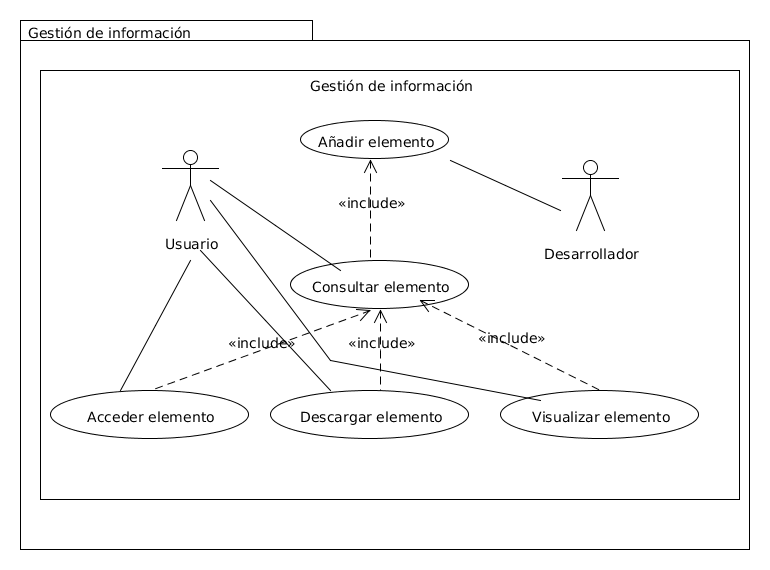
\includegraphics[width=1\textwidth]{imagenes/diagrama_casos_uso.png}
\end{figure}

%\section{Glosario de términos}

%Poner aquí o en otro apartado más adelante.
%
%\chapter{Planificación}

\section{Fases y entregas}

\subsection{Fases}

Como este va a ser un proyecto que ya cuenta con un trabajo previo realizado, la fase inicial de gestión va a ser muy breve
porque se parte de que ya se han realizado varias reuniones y el proyecto está parcialmente funcionando, por lo que no se parte
de cero, es una ampliación de un proyecto inicial.

\begin{itemize}
  \item \textbf{Fase 1:} Especificaciones del proyecto
  \item \textbf{Fase 2:} Planificación
  \item \textbf{Fase 3:} Análisis y diseño
  \item \textbf{Fase 4:} Implementación
  \item \textbf{Fase 5:} Pruebas
  \item \textbf{Fase 6:} Documentación
\end{itemize}

\subsection{Lista de entregas}

Se harán una serie de breves informes sobre el contenido de cada una de las fases de planificación del proyecto.

\begin{itemize}
  \item \textbf{Fase 1:} Especificación del proyecto.
  \begin{itemize}
    \item Descripción: Se establecen los objetivos a cumplir para que el desarrollo del proyecto se considere completado.
    \item Tipo: informe.
  \end{itemize}
  \newpage
  \item \textbf{Fase 2:} Planificación.
  \begin{itemize}
    \item Descripción: Se desarrolla la documentación con toda la planificación del desarrollo del proyecto.
    \item Tipo: informe.
  \end{itemize}
  \item \textbf{Fase 3:} Análisis y diseño.
  \begin{itemize}
    \item Descripción: Todos los aspectos del proyectos son analizados para concretar la forma de desarrollarlo.
    \item Tipo: informe.
  \end{itemize}
  \item \textbf{Fase 4:} Implementación.
  \begin{itemize}
    \item Descripción: Con el proyecto ya planificado y diseña se pasa programar todo lo necesario para cumplir los objetivos.
    \item Tipo: software.
  \end{itemize}
  \item \textbf{Fase 5:} Pruebas.
  \begin{itemize}
    \item Descripción: Una vez este todo programado, se pasa a validar con diferentes procedimientos que el proyecto funciona
    correctamente tomando como referentes unas métricas propias.
    \item Tipo: informe y software.
  \end{itemize}
  \item \textbf{Fase 6:} Documentación.
  \begin{itemize}
    \item Descripción: Para finalizar el proyecto se realiza toda la documentación informativa y explicativa.
    \item Tipo: informe.
  \end{itemize}
\end{itemize}

\section{Estructura de Descomposición del Trabajo}

El diagrama de Estructura de Descomposición del Trabajo (figura 3.1) es una descomposición jerárquica de las diferentes fases y 
entregas en las que está planificado el proyecto.

\newpage
\section{Lista de actividades}

Las actividades que se vayan a desarrollar en cada una de las fases para cada una de las entregas se va a listar junto con una 
estimación del tiempo que deberían tomar en ser cumplidas.

\begin{itemize}
   \item \textbf{Especificaciones del proyecto:}
   \begin{itemize}
    \item Determinación de objetivos.
    \item Determinación de requisitos.
    \item \underline{\textit{Estimación: 9 horas}}
    \end{itemize}
\end{itemize}

\begin{itemize}
   \item \textbf{Planificación:}
   \begin{itemize}
    \item Lista de actividades.
    \item Recursos humanos.
    \item Presupuesto.
    \item Temporización.
    \item \underline{\textit{Estimación: 18 horas}}
   \end{itemize}
\end{itemize}

\begin{itemize}
   \item \textbf{Análisis y diseño:}
   \begin{itemize}
    \item Análisis de requisitos.
    \item Diagramas.
    \item Metodología de desarrollo.
    \item Descripción estructural.
    \item \underline{\textit{Estimación: 36 horas}}
   \end{itemize}
\end{itemize}

\begin{itemize}
 \item \textbf{Implementación:}
 \begin{itemize}
  \item Herramientas seleccionadas.
  \item Solucionar problema de generación de páginas.
  \item Implementar tests unitarios.
  \item Implementar test de cobertura.
  \item Introducir integración continua.
  \item Agregar despliegue automático.
  \item Actualizar aprovisionamiento.
  \item \underline{\textit{Estimación: 90 horas}}
 \end{itemize}
\end{itemize}

\newpage
\begin{itemize}
 \item \textbf{Pruebas:}
 \begin{itemize}
  \item Pruebas de software.
  \item Pruebas de carga.
  \item \underline{\textit{Estimación: 30 horas}}
 \end{itemize}
\end{itemize}

\begin{itemize}
 \item \textbf{Documentación:}
 \begin{itemize}
  \item Documentación de la aplicación.
  \item Manual de usuario.
  \item Documentación del proyecto.
  \item \underline{\textit{Estimación: 30 horas}}
 \end{itemize}
\end{itemize}

\section{Recursos humanos}

Como este es un proyecto que comenzó su desarrollo en la Oficina de Software Libre de la Universidad de Granada, cuento con el
apoyo de todos sus colaboradores, además del resto de becarios que se encuentran realizando prácticas en empresa en ella
como es mi situación actual, además, siendo el tutor de este proyecto el director de la propia oficina.

\section{Presupuesto}

Una de las ventajas de usar software libre es que no es necesario adquirir licencias por las que haya que pagar para realizar 
su uso, como todas las herramientas que usen (al igual que las que se generen) serán software libre, el coste en software para 
el desarrollo será cero.

\bigskip

El único recurso necesario es el servidor en que estará instalada el portal, servidor ya que adquirido anteriormente, por
lo que tampoco es necesario considerarlo un gasto a afrontar de cara al desarrollo.

\section{Temporización}

Para percibir de forma más visual la planificación temporal de las tareas se incluyen la figura 3.2 con una tabla indicando los
plazos de cada tarear y la figura 3.3 con un diagrama de Gantt de dichas tareas.
\newpage

\begin{figure}[!ht]
  \begin{center}
    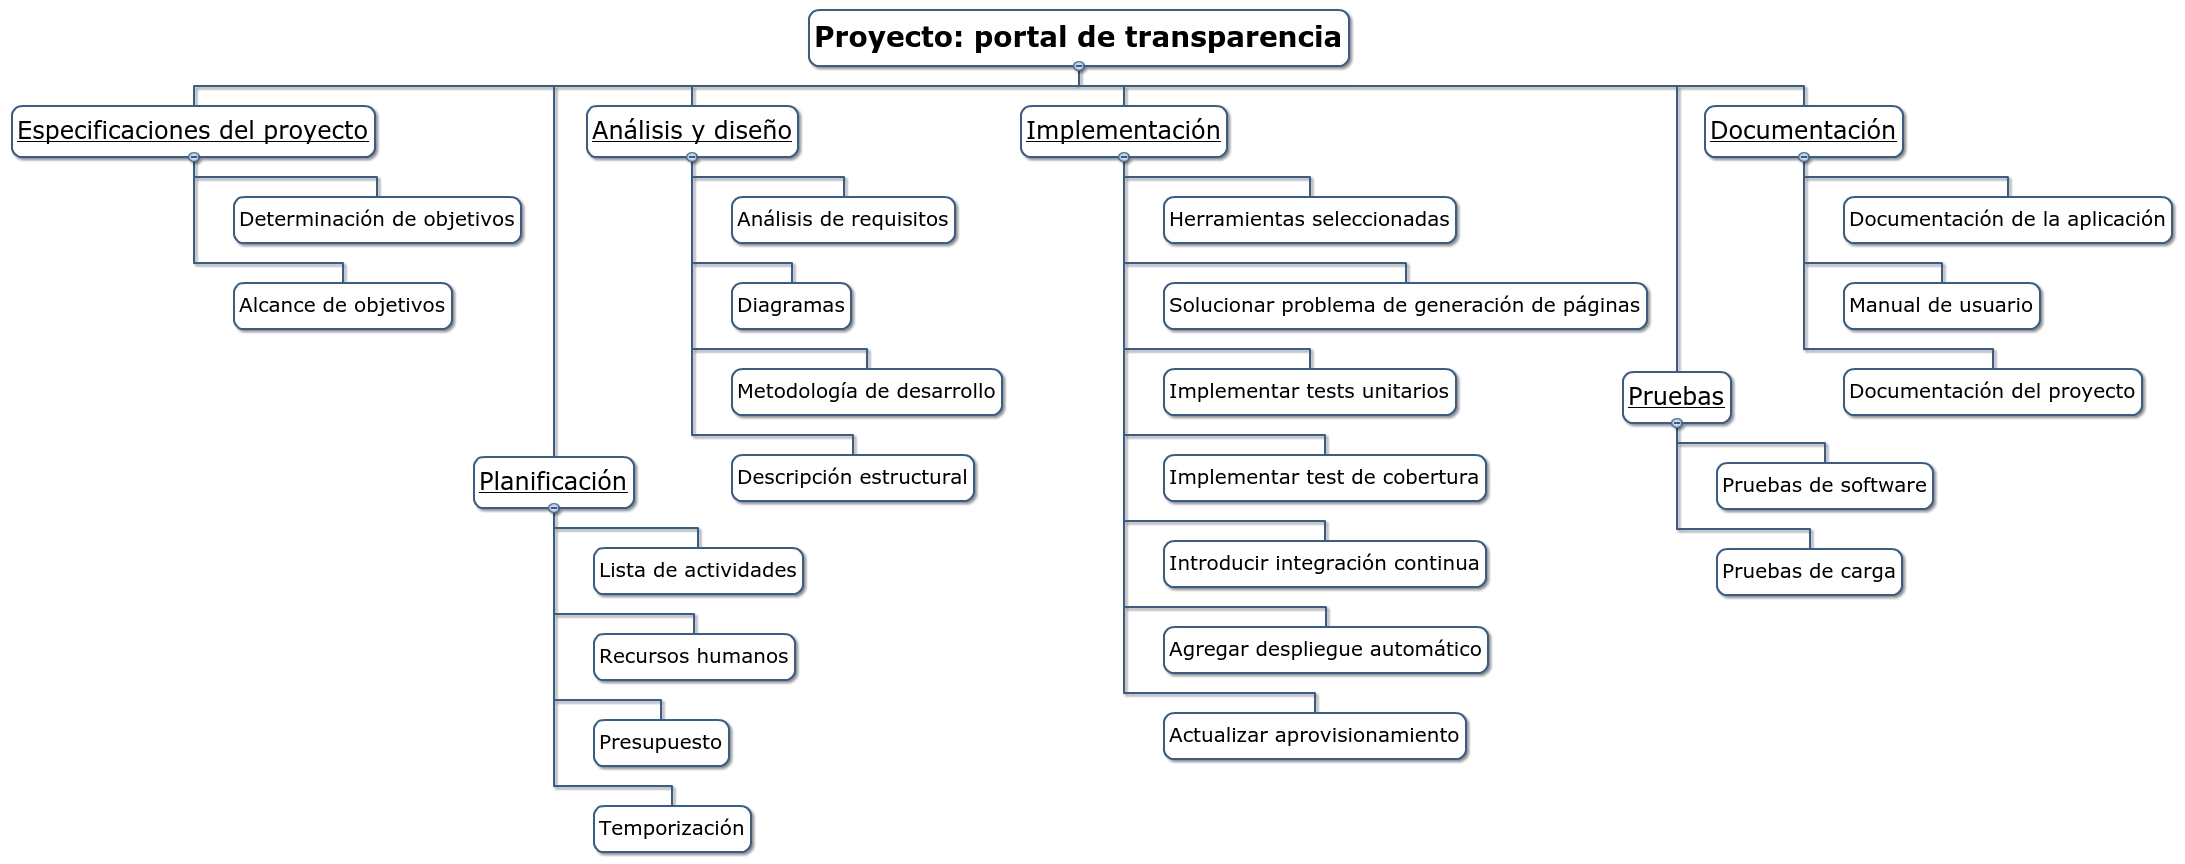
\includegraphics[scale=0.25,angle=90]{imagenes/diagrama_edt.png}
    \caption{Diagrama de Estructura de Descomposición de Trabajo}
    \label{fig:diag_edt}
  \end{center}
\end{figure}

\newpage
\begin{figure}[!ht]
  \begin{center}
    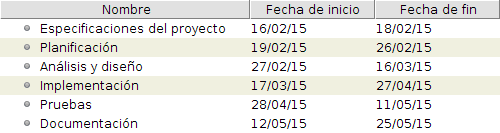
\includegraphics[width=1\textwidth]{imagenes/tempo_tareas.png}
    \caption{Temporización de las tareas}
    \label{fig:tempo_tareas}
  \end{center}
\end{figure}

% \begin{table}[!ht]
%   \begin{center}
%     \begin{tabular}{|l|l|l|}
%       \hline
%       \multicolumn{1}{|c|}{{\bf Nombre}} & \multicolumn{1}{c|}{{\bf Fecha de inicio}} & \multicolumn{1}{c|}{{\bf Fecha de fin}} \\ \hline
%       Especificaciones del proyecto      & 16/02/15                                   & 18/02/15                                \\ \hline
%       Planificación                      & 19/02/15                                   & 26/02/15                                \\ \hline
%       Análisis y diseño                  & 27/02/15                                   & 16/03/15                                \\ \hline
%       Implementación                     & 17/03/15                                   & 27/04/15                                \\ \hline
%       Pruebas                            & 28/04/15                                   & 11/05/15                                \\ \hline
%       Documentación                      & 12/05/15                                   & 25/05/15                                \\ \hline
%     \end{tabular}
%     \caption{Temporización de las tareas}
%     \label{table:tempo_tareas}
%   \end{center}
% \end{table}

\begin{figure}[!ht]
  \begin{center}
    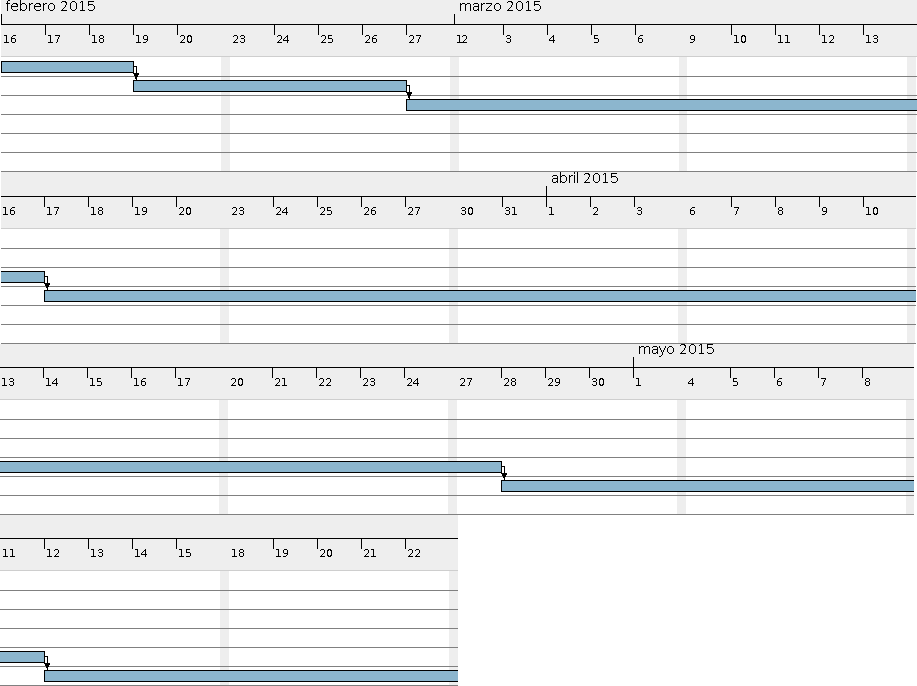
\includegraphics[width=1\textwidth]{imagenes/diagrama_gantt.png}
    \caption{Diagrama de Gantt}
    \label{fig:diag_edt}
  \end{center}
\end{figure}
%
%\chapter{Análisis}

\section{Análisis de requisitos}

Todo software se desarrolla para cubrir una necesidad, por lo que en este apartado vamos a describir los requisitos que se estiman necesarios para cubrir los objetivos propuestos.

\subsection{Descripción de los actores}

Los actores implicados serán dos: el \textbf{desarrollador} y el \textbf{usuario}.

\bigskip
El \textbf{desarrollador} será el encargado de solucionar los problemas de visualización de los datos en el portal, además de portar el desarrollo actual del portal a un entorno de desarrollo continuo. También asumirá la administración del portal ya que este tipo de rol está muy integrado con las labores de despliegue en el desarrollo continuo.

\bigskip
El \textbf{usuario} de la aplicación será cualquier persona que tenga interés por conocer datos internos de la Universidad de Granada fácilmente. El usuario no pertenece a ningún público objetivo concreto, por lo que no se tiene que considerar que tenga una experiencia previa en navegador por sitios web.

\subsection{Requisitos funcionales}

Los requisitos funcionales son las características que tiene que implementar el sistema para cubrir todas las necesidades de los distintos usuarios.

\bigskip
Al usuario lo único que le interesa es ver una página web estática con la información que desea 
consultar, para ello el desarrollador deberá hacer que sea posible que se generen siempre las tablas con los elementos de información. 

\bigskip
Por otra parte, el desarrollador quiere integrar el sistema en un desarrollo continuo, por lo que añadirá tests unitarios, test de cobertura, integración continua, despliegue automático y aprovisionamiento con tal fin.

\begin{itemize}
  \item \textbf{RF-1.} Administración portal:
    \begin{itemize}
    \item \textbf{RF-1.1.} Automatizar inicio del servidor del portal.
    \end{itemize}
\end{itemize}

\begin{itemize}
  \item \textbf{RF-2.} Acceso información:
    \begin{itemize}
    \item \textbf{RF-2.1.} Consultar información de Administración.
    \item \textbf{RF-2.1.} Consultar información de Docencia.
    \item \textbf{RF-2.1.} Consultar información de Gestión e Investigación.
    \item \textbf{RF-2.1.} Consultar información de Normativa Legal.
    \end{itemize}
\end{itemize}

\begin{itemize}
  \item \textbf{RF-3.} Pruebas de software:
  \begin{itemize}
    \item \textbf{RF-3.1.} Realizar tests unitarios.
    \item \textbf{RF-3.2.} Realizar test de cobertura.
    \item \textbf{RF-3.2.} Usar integración continua.
    \end{itemize}
\end{itemize}

\begin{itemize}
  \item \textbf{RF-4.} Configuración automática:
  \begin{itemize}
    \item \textbf{RF-4.1.} Usar despliegue automático.
    \item \textbf{RF-4.2.} Usar aprovisionamiento.
    \end{itemize}
\end{itemize}

\subsection{Requisitos no funcionales}

Los requisitos no funcionales son las características propias del desarrollo, pero que no tienen que estar relacionadas con su funcionalidad.

\begin{itemize}
  \item \textbf{RN-1.} Toda la programación del portal se hará en Node.js y los módulos que se usen deben ser instalables a través de su gestor de paquetes NPM.
  \item \textbf{RN-2.} El portal se iniciará y se detendrá mediante scripts lanzados con NPM.
  \item \textbf{RN-3.} Para iniciar la ejecución del portal es necesario que reciba el puerto de escucha del servidor y la dirección de acceso.
  \item \textbf{RN-4.} Todos los módulos se ejecutarán desde scripts lanzamos con NPM.
  \item \textbf{RN-5.} Los tests unitarios se realizarán en base a comportamientos esperados y valores de estados
  recibidos como contestación a las peticiones que se realicen al portal.
  \item \textbf{RN-6.} Los tests unitarios tienen que recibir las páginas del portal para ejecutarse.
  \item \textbf{RN-7.} El test de cobertura tiene que tener una automatización integrable con los tests unitarios. 
  \item \textbf{RN-8.} La integración continua se ejecutará automáticamente con cada cambio que se haga en la programación del portal.
  \item \textbf{RN-9.} El despliegue automático se realizará mediante conexiones SSH.
  \item \textbf{RN-10.} Tanto para el despliegue automático como para el aprovisionamiento es necesario indicar el usuario que lo realiza y el destino en el que se realiza.
\end{itemize}

\subsection{Requisitos de información}

Los requisitos de información se refieren a la información que es necesaria almacenar en el sistema. La única información relevante que se va a almacenar son los datos descriptivos y de enlace de cada uno de los elementos del portal OpenData UGR que se van a mostrar en UGR Transparente.

\begin{itemize}
  \item \textbf{RI-1.} Datos abiertos.
  \begin{itemize}
    \item Información sobre cada uno de los elementos que se van a mostrar en el portal de transparencia como datos abiertos.
    \item Contenido: nombre, categoría, conjunto de datos, enlace a OpenData UGR, enlace al recurso.
  \end{itemize}
\end{itemize}

\section{Modelos de casos de uso}

Aunque ya se ha indicado que la parte funcional ya se encuentra implementada de forma previa a este proyecto, se van a incluir unos modelos de caso de uso simples para dar un visión más clara del funcionamiento general del portal UGR Transparente.

\newpage
\subsection{Descripción básica de actores}

\begin{itemize}
  \item \textbf{Ac-1.} Desarrollador
  \begin{itemize}
   \item Descripción: Encargado del desarrollo y administración del portal.
   \item Características: Su trabajo está en el lado del servidor que genera la página, nunca trabaja desde el lado del cliente.
   \item Relaciones: Ninguna.
   \item Atributos: Ninguno.
   \item Comentarios: Es el encargado de que la información se muestre en el portal y de añadir funcionalidades al portal.
  \end{itemize}
  
  \item \textbf{Ac-2.} Usuario
  \begin{itemize}
   \item Descripción: Persona que usa el portal para consultar datos.
   \item Características: Es el usuario común que accederá a la página.
   \item Relaciones: Ninguna.
   \item Atributos: Ninguno.
   \item Comentarios: El usuario no es necesario que tenga ningún conocimiento previo al uso del portal, simplemente accederá y consultará los datos que sean de su interes.
  \end{itemize}
\end{itemize}

\subsection{Descripción casos de uso}

\begin{itemize}
  \item \textbf{CU-1.} Inicio automático del servidor del portal
  \begin{itemize}
    \item Actores: Desarrollador
    \item Tipo: Primario, esencial
    \item Referencias:
    \item Precondición: El servidor esté detenido.
    \item Postcondición: El portal será accesible públicamente.
    \item Autor: \autor
    \item Versión: 1.0
    \item Propósito: Iniciar el servidor del portal UGR Transparente.
    \item Resumen: Cuando se ejecuta el script de inicio de la aplicación, arranca el servidor y el portal será accesible desde Internet.
    \begin{table}[!ht]
      \begin{center}
	\begin{tabular}{|l|l|l|l|}
	  \hline
	  \multicolumn{4}{|c|}{{\bf Curso normal}}
	  \\ \hline
	  \multicolumn{2}{|c|}{{\bf Actor}} & \multicolumn{2}{c|}{{\bf Sistema}}
	  \\ \hline
	  {\it 1} & 
	  \begin{tabular}[c]{@{}l@{}}
	    Desarrollador: da orden de\\
	    que se inicie el servidor\\
	    del portal.
	  \end{tabular} &
	  &
	  \\ \hline
	  &
	  &
	  {\it 2a} &
	  \begin{tabular}[c]{@{}l@{}}
	    Comprueba que el servidor\\
	    está detenido y lo inicia\\
	    para que el portal esté\\
	    operativo.
	  \end{tabular}
	  \\ \hline
	\end{tabular}
	\caption{Curso normal de CU-1. Inicio automático del servidor del portal}
	\label{table:cn_cu_1}
      \end{center}
    \end{table}
    \begin{table}[!ht]
      \begin{center}
	\begin{tabular}{|l|l|}
	  \hline
	  \multicolumn{2}{|c|}{{\bf Curso alterno}}
	  \\ \hline
	  {\it 2b} &
	  \begin{tabular}[c]{@{}l@{}}
	    Si el servidor está funcionando, no se ejecuta el script de\\
	    inicio del servidor.
	  \end{tabular}\\
	  \hline
	\end{tabular}
	\caption{Curso alterno de CU-1. Inicio automático del servidor del portal}
	\label{table:ca_cu_1}
      \end{center}
    \end{table}
  \end{itemize}
 
  \newpage
  \item \textbf{CU-2.} Consultar información de Administración
  \begin{itemize}
    \item Actores: Usuario
    \item Tipo: Primario, esencial
    \item Referencias:
    \item Precondición: Existan archivos con los datos abiertos.
    \item Postcondición:
    \item Autor: \autor
    \item Versión: 1.0
    \item Propósito: El usuario consulta datos de administración en el portal UGR Transparente.
    \item Resumen: El usuario que accede al portal de transparencia selecciona la sección de ``Administración'' y consulta la información de sus subsecciones.
    \begin{table}[!ht]
      \begin{center}
	\begin{tabular}{|l|l|l|l|}
	  \hline
	  \multicolumn{4}{|c|}{{\bf Curso normal}}
	  \\ \hline
	  \multicolumn{2}{|c|}{{\bf Actor}} & \multicolumn{2}{c|}{{\bf Sistema}}
	  \\ \hline
	  {\it 1} & 
	  \begin{tabular}[c]{@{}l@{}}
	    Usuario: consulta la información\\
	    de Administración publicada en el\\
	    portal.
	  \end{tabular} &
	  &
	  \\ \hline
	  &
	  &
	  {\it 2} &
	  \begin{tabular}[c]{@{}l@{}}
	    Se generan las tablas con\\
	    todos los elementos de\\
	    información de la sección\\
	    Administración.
	  \end{tabular}
	  \\ \hline
	  &
	  &
	  {\it 3} &
	  \begin{tabular}[c]{@{}l@{}}
	    Se muestran en la página\\
	    todos las tablas generadas\\
	    con los elementos de\\
	    información.
	  \end{tabular}
	  \\ \hline
	\end{tabular}
	\caption{Curso normal de CU-2. Consultar información de Administración}
	\label{table:cn_cu_2}
      \end{center}
    \end{table}
  \end{itemize}
  
  \newpage
  \item \textbf{CU-3.} Consultar información de Docencia
  \begin{itemize}
    \item Actores: Usuario
    \item Tipo: Primario, esencial
    \item Referencias:
    \item Precondición: Existan archivos con los datos abiertos.
    \item Postcondición:
    \item Autor: \autor
    \item Versión: 1.0
    \item Propósito: El usuario consulta datos de administración en el portal UGR Transparente.
    \item Resumen: El usuario que accede al portal de transparencia selecciona la sección de ``Docencia'' y consulta la información de sus subsecciones.
    \begin{table}[!ht]
      \begin{center}
	\begin{tabular}{|l|l|l|l|}
	  \hline
	  \multicolumn{4}{|c|}{{\bf Curso normal}}
	  \\ \hline
	  \multicolumn{2}{|c|}{{\bf Actor}} & \multicolumn{2}{c|}{{\bf Sistema}}
	  \\ \hline
	  {\it 1} & 
	  \begin{tabular}[c]{@{}l@{}}
	    Usuario: consulta la información\\
	    de Docencia publicada en el\\
	    portal.
	  \end{tabular} &
	  &
	  \\ \hline
	  &
	  &
	  {\it 2} &
	  \begin{tabular}[c]{@{}l@{}}
	    Se generan las tablas con\\
	    todos los elementos de\\
	    información de la sección\\
	    Docencia.
	  \end{tabular}
	  \\ \hline
	  &
	  &
	  {\it 3} &
	  \begin{tabular}[c]{@{}l@{}}
	    Se muestran en la página\\
	    todos las tablas generadas\\
	    con los elementos de\\
	    información.
	  \end{tabular}
	  \\ \hline
	\end{tabular}
	\caption{Curso normal de CU-3. Consultar información de Docencia}
	\label{table:cn_cu_3}
      \end{center}
    \end{table}
  \end{itemize}
  
  \newpage
  \item \textbf{CU-4.} Consultar información de Gestión e Investigación
  \begin{itemize}
    \item Actores: Usuario
    \item Tipo: Primario, esencial
    \item Referencias:
    \item Precondición: Existan archivos con los datos abiertos.
    \item Postcondición:
    \item Autor: \autor
    \item Versión: 1.0
    \item Propósito: El usuario consulta datos de administración en el portal UGR Transparente.
    \item Resumen: El usuario que accede al portal de transparencia selecciona la sección de ``Gestión e Investigación'' y consulta la información de sus subsecciones.
    \begin{table}[!ht]
      \begin{center}
	\begin{tabular}{|l|l|l|l|}
	  \hline
	  \multicolumn{4}{|c|}{{\bf Curso normal}}
	  \\ \hline
	  \multicolumn{2}{|c|}{{\bf Actor}} & \multicolumn{2}{c|}{{\bf Sistema}}
	  \\ \hline
	  {\it 1} & 
	  \begin{tabular}[c]{@{}l@{}}
	    Usuario: consulta la información\\
	    de Gestión e Investigación publicada\\
	    en el portal.
	  \end{tabular} &
	  &
	  \\ \hline
	  &
	  &
	  {\it 2} &
	  \begin{tabular}[c]{@{}l@{}}
	    Se generan las tablas con\\
	    todos los elementos de\\
	    información de la sección\\
	    Gestión e Investigación.
	  \end{tabular}
	  \\ \hline
	  &
	  &
	  {\it 3} &
	  \begin{tabular}[c]{@{}l@{}}
	    Se muestran en la página\\
	    todos las tablas generadas\\
	    con los elementos de\\
	    información.
	  \end{tabular}
	  \\ \hline
	\end{tabular}
	\caption{Curso normal de CU-4. Consultar información de Gestión e Investigación}
	\label{table:cn_cu_4}
      \end{center}
    \end{table}
  \end{itemize}
  
  \newpage
  \item \textbf{CU-5.} Consultar información de Normativa Legal
  \begin{itemize}
    \item Actores: Usuario
    \item Tipo: Primario, esencial
    \item Referencias:
    \item Precondición: Existan archivos con los datos abiertos.
    \item Postcondición:
    \item Autor: \autor
    \item Versión: 1.0
    \item Propósito: El usuario consulta datos de administración en el portal UGR Transparente.
    \item Resumen: El usuario que accede al portal de transparencia selecciona la sección de ``Normativa Legal'' y consulta la información de sus subsecciones.
    \begin{table}[!ht]
      \begin{center}
	\begin{tabular}{|l|l|l|l|}
	  \hline
	  \multicolumn{4}{|c|}{{\bf Curso normal}}
	  \\ \hline
	  \multicolumn{2}{|c|}{{\bf Actor}} & \multicolumn{2}{c|}{{\bf Sistema}}
	  \\ \hline
	  {\it 1} & 
	  \begin{tabular}[c]{@{}l@{}}
	    Usuario: consulta la información\\
	    de Normativa Legal publicada en el\\
	    portal.
	  \end{tabular} &
	  &
	  \\ \hline
	  &
	  &
	  {\it 2} &
	  \begin{tabular}[c]{@{}l@{}}
	    Se generan las tablas con\\
	    todos los elementos de\\
	    información de la sección\\
	    Normativa Legal.
	  \end{tabular}
	  \\ \hline
	  &
	  &
	  {\it 3} &
	  \begin{tabular}[c]{@{}l@{}}
	    Se muestran en la página\\
	    todos las tablas generadas\\
	    con los elementos de\\
	    información.
	  \end{tabular}
	  \\ \hline
	\end{tabular}
	\caption{Curso normal de CU-5. Consultar información de Normativa Legal}
	\label{table:cn_cu_5}
      \end{center}
    \end{table}
  \end{itemize}
 
  \newpage
  \item \textbf{CU-6.} Realizar tests unitarios
  \begin{itemize}
    \item Actores: Desarrollador
    \item Tipo: Primario, esencial
    \item Referencias:
    \item Precondición: Existan tests unitarios.
    \item Postcondición: 
    \item Autor: \autor
    \item Versión: 1.0
    \item Propósito: Realizar tests unitarios para comprobar las funcionalidades de la aplicación.
    \item Resumen: Cada vez que se añadan nuevas páginas o funcionalidades al portal, se comprueba que funcionan correctamente.
    \begin{table}[!ht]
      \begin{center}
	\begin{tabular}{|l|l|l|l|}
	  \hline
	  \multicolumn{4}{|c|}{{\bf Curso normal}}
	  \\ \hline
	  \multicolumn{2}{|c|}{{\bf Actor}} & \multicolumn{2}{c|}{{\bf Sistema}}
	  \\ \hline
	  {\it 1} & 
	  \begin{tabular}[c]{@{}l@{}}
	    Desarrollador: da orden de\\
	    ejecutar los tests unitarios.
	  \end{tabular} &
	  &
	  \\ \hline
	  &
	  &
	  {\it 2a} &
	  \begin{tabular}[c]{@{}l@{}}
	    Comprueba que hay tests\\
	    unitarios y los ejecuta.\\
	  \end{tabular}
	  \\ \hline
	\end{tabular}
	\caption{Curso normal de CU-6. Realizar tests unitarios}
	\label{table:cn_cu_6}
      \end{center}
    \end{table}
    \begin{table}[!ht]
      \begin{center}
	\begin{tabular}{|l|l|}
	  \hline
	  \multicolumn{2}{|c|}{{\bf Curso alterno}}
	  \\ \hline
	  {\it 2b} &
	  \begin{tabular}[c]{@{}l@{}}
	    Si no hay tests unitarios creados, el sistema no hace nada.
	  \end{tabular}\\
	  \hline
	\end{tabular}
	\caption{Curso alterno de CU-6. Realizar tests unitarios}
	\label{table:ca_cu_6}
      \end{center}
    \end{table}
  \end{itemize}
 
  \newpage
  \item \textbf{CU-7.} Realizar tests de cobertura
  \begin{itemize}
    \item Actores: Desarrollador
    \item Tipo: Primario, esencial
    \item Referencias: (CU-6.) Realizar tests unitarios
    \item Precondición: Existan tests unitarios.
    \item Postcondición: 
    \item Autor: \autor
    \item Versión: 1.0
    \item Propósito: Realizar test de cobertura para comprobar calidad de los tests unitarios.
    \item Resumen: Para comprobar si los tests unitarios cumplen correctamente con su función se analiza el porcentaje del código que está cubierto por los mismos.
    \begin{table}[!ht]
      \begin{center}
	\begin{tabular}{|l|l|l|l|}
	  \hline
	  \multicolumn{4}{|c|}{{\bf Curso normal}}
	  \\ \hline
	  \multicolumn{2}{|c|}{{\bf Actor}} & \multicolumn{2}{c|}{{\bf Sistema}}
	  \\ \hline
	  {\it 1} & 
	  \begin{tabular}[c]{@{}l@{}}
	    Desarrollador: da orden de\\
	    ejecutar test de cobertura.
	  \end{tabular} &
	  &
	  \\ \hline
	  &
	  &
	  {\it 2a} &
	  \begin{tabular}[c]{@{}l@{}}
	    Comprueba que hay tests\\
	    unitarios y los ejecuta.\\
	  \end{tabular}
	  \\ \hline
	  &
	  &
	  {\it 3} &
	  \begin{tabular}[c]{@{}l@{}}
	    Se ejecuta el test de \\
	    cobertura en base a los\\
	    tests unitarios ejecutados.
	  \end{tabular}
	  \\ \hline
	\end{tabular}
	\caption{Curso normal de CU-7. Realizar test de cobertura}
	\label{table:cn_cu_7}
      \end{center}
    \end{table}
    \begin{table}[!ht]
      \begin{center}
	\begin{tabular}{|l|l|}
	  \hline
	  \multicolumn{2}{|c|}{{\bf Curso alterno}}
	  \\ \hline
	  {\it 2b} &
	  \begin{tabular}[c]{@{}l@{}}
	    Si no hay tests unitarios creados, el sistema no hace nada.
	  \end{tabular}\\
	  \hline
	\end{tabular}
	\caption{Curso alterno de CU-7. Realizar test de cobertura}
	\label{table:ca_cu_7}
      \end{center}
    \end{table}
  \end{itemize}
 
  \newpage
  \item \textbf{CU-8.} Usar integración continua
  \begin{itemize}
    \item Actores: Desarrollador
    \item Tipo: Primario, esencial
    \item Referencias: (CU-5.) Realizar tests unitarios
    \item Precondición: Existan test unitarios.
    \item Postcondición: Se genera un informe con el resultado de los tests unitarios.
    \item Autor: \autor
    \item Versión: 1.0
    \item Propósito: Comprobar si los cambios en la aplicación provocan errores.
    \item Resumen: Cuando se efectúan cambios en la aplicación automáticamente se ejecutan los tests unitarios para comprobar si los cambios introducidos provocan conflictos en la plataforma.
    \begin{table}[!ht]
      \begin{center}
	\begin{tabular}{|l|l|l|l|}
	  \hline
	  \multicolumn{4}{|c|}{{\bf Curso normal}}
	  \\ \hline
	  \multicolumn{2}{|c|}{{\bf Actor}} & \multicolumn{2}{c|}{{\bf Sistema}}
	  \\ \hline
	  {\it 1} & 
	  \begin{tabular}[c]{@{}l@{}}
	    Desarrollador: guardar\\
	    cambios en el repositorio.
	  \end{tabular} &
	  &
	  \\ \hline
	  &
	  &
	  {\it 2a} &
	  \begin{tabular}[c]{@{}l@{}}
	    Comprueba que hay tests\\
	    unitarios y comienza la\\
	    verificación de la\\
	    integración continua.
	  \end{tabular}
	  \\ \hline
	  &
	  &
	  {\it 3} &
	  \begin{tabular}[c]{@{}l@{}}
	    Ejecuta los tests unitarios\\
	    para cada entorno definido.
	  \end{tabular}
	  \\ \hline
	\end{tabular}
	\caption{Curso normal de CU-8. Usar integración continua}
	\label{table:cn_cu_8}
      \end{center}
    \end{table}
    \begin{table}[!ht]
      \begin{center}
	\begin{tabular}{|l|l|}
	  \hline
	  \multicolumn{2}{|c|}{{\bf Curso alterno}}
	  \\ \hline
	  {\it 2b} &
	  \begin{tabular}[c]{@{}l@{}}
	    Si no hay tests unitarios creados, el sistema no hace nada.
	  \end{tabular}\\
	  \hline
	\end{tabular}
	\caption{Curso alterno de CU-8. Usar integración continua}
	\label{table:ca_cu_8}
      \end{center}
    \end{table}
  \end{itemize}
 
  \newpage
  \item \textbf{CU-.9 } Usar despliegue automático
  \begin{itemize}
    \item Actores: Desarrollador
    \item Tipo: Primario, esencial
    \item Referencias: (CU-1.) Iniciar plataforma
    \item Precondición: 
    \item Postcondición: Los cambios introducidos son aplicados en la plataforma.
    \item Autor: \autor
    \item Versión: 1.0
    \item Propósito: Aplicar automáticamente los cambios realizados a la aplicación. 
    \item Resumen: Para no tener que acceder manualmente al servidor de la plataforma y tener que desplegar los cambios introducidos, desde el entorno de desarrollo desplegamos automáticamente los cambios en el servidor.
    \begin{table}[!ht]
      \begin{center}
	\begin{tabular}{|l|l|l|l|}
	  \hline
	  \multicolumn{4}{|c|}{{\bf Curso normal}}
	  \\ \hline
	  \multicolumn{2}{|c|}{{\bf Actor}} & \multicolumn{2}{c|}{{\bf Sistema}}
	  \\ \hline
	  {\it 1} & 
	  \begin{tabular}[c]{@{}l@{}}
	    Desarrollador: ordenar\\
	    despliegue automático.
	  \end{tabular} &
	  &
	  \\ \hline
	  &
	  &
	  {\it 2} &
	  \begin{tabular}[c]{@{}l@{}}
	    Conectar al servidor.
	  \end{tabular}
	  \\ \hline
	  &
	  &
	  {\it 3} &
	  \begin{tabular}[c]{@{}l@{}}
	    Crear copia de seguridad.
	  \end{tabular}
	  \\ \hline
	  &
	  &
	  {\it 4a} &
	  \begin{tabular}[c]{@{}l@{}}
	    Comprobar si hay cambios en\\
	    el repositorio de la\\
	    plataforma y descargarlos\\
	    en dicho caso.
	  \end{tabular}
	  \\ \hline
	  &
	  &
	  {\it 5} &
	  \begin{tabular}[c]{@{}l@{}}
	    Iniciar la plataforma con\\
	    los cambios aplicados.
	  \end{tabular}
	  \\ \hline
	\end{tabular}
	\caption{Curso normal de CU-9. Usar despliegue automático}
	\label{table:cn_cu_9}
      \end{center}
    \end{table}
    \begin{table}[!ht]
      \begin{center}
	\begin{tabular}{|l|l|}
	  \hline
	  \multicolumn{2}{|c|}{{\bf Curso alterno}}
	  \\ \hline
	  {\it 4b} &
	  \begin{tabular}[c]{@{}l@{}}
	    Si no hay cambios aplicables, se continua con el proceso.
	  \end{tabular}\\
	  \hline
	\end{tabular}
	\caption{Curso alterno de CU-9. Usar despliegue automático}
	\label{table:ca_cu_9}
      \end{center}
    \end{table}
  \end{itemize}
 
  \newpage
  \item \textbf{CU-.10} Usar aprovisionamiento
  \begin{itemize}
    \item Actores: Desarrollador
    \item Tipo: Primario, esencial
    \item Referencias: (CU-1.) Iniciar plataforma
    \item Precondición: 
    \item Postcondición: El portal queda instalado en la infraestructura seleccionada.
    \item Autor: \autor
    \item Versión: 1.0
    \item Propósito: Instalar automáticamente el portal en una infraestructura dada.
    \item Resumen: Se instalarán automáticamente todos los elementos necesarios para poner en funcionamiento el portal en cualquier infraestructura que se indique.
    \begin{table}[!ht]
      \begin{center}
	\begin{tabular}{|l|l|l|l|}
	  \hline
	  \multicolumn{4}{|c|}{{\bf Curso normal}}
	  \\ \hline
	  \multicolumn{2}{|c|}{{\bf Actor}} & \multicolumn{2}{c|}{{\bf Sistema}}
	  \\ \hline
	  {\it 1} & 
	  \begin{tabular}[c]{@{}l@{}}
	    Desarrollador: ordenar\\
	    despliegue automático.
	  \end{tabular} &
	  &
	  \\ \hline
	  &
	  &
	  {\it 2} &
	  \begin{tabular}[c]{@{}l@{}}
	    Conectar al servidor.
	  \end{tabular}
	  \\ \hline
	  &
	  &
	  {\it 3} &
	  \begin{tabular}[c]{@{}l@{}}
	    Comprobar aplicación necesaria.
	  \end{tabular}
	  \\ \hline
	  &
	  &
	  {\it 4a} &
	  \begin{tabular}[c]{@{}l@{}}
	    Se comprueba si la aplicación\\
	    necesaria está instalada,\\
	    instalándola en caso de que\\
	    no lo esté.
	  \end{tabular}
	  \\ \hline
	  &
	  &
	  {\it 5} &
	  \begin{tabular}[c]{@{}l@{}}
	    Descarga la plataforma desde\\
	    el repositorio.
	  \end{tabular}
	  \\ \hline
	  &
	  &
	  {\it 6} &
	  \begin{tabular}[c]{@{}l@{}}
	    Instalar todas las dependencias\\
	    de la plataforma.
	  \end{tabular}
	  \\ \hline
	  &
	  &
	  {\it 7} &
	  \begin{tabular}[c]{@{}l@{}}
	    Se establecen los parámetros de\\
	    acceso al portal desde Internet.
	  \end{tabular}
	  \\ \hline
	  &
	  &
	  {\it 8} &
	  \begin{tabular}[c]{@{}l@{}}
	    Con todo preparado, se inicia\\
	    la plataforma.
	  \end{tabular}
	  \\ \hline
	\end{tabular}
	\caption{Curso normal de CU-10. Usar aprovisionamiento}
	\label{table:cn_cu_10}
      \end{center}
    \end{table}
    \begin{table}[!ht]
      \begin{center}
	\begin{tabular}{|l|l|}
	  \hline
	  \multicolumn{2}{|c|}{{\bf Curso alterno}}
	  \\ \hline
	  {\it 4b} &
	  \begin{tabular}[c]{@{}l@{}}
	    Si la aplicación está instalada, se continua con el proceso.
	  \end{tabular}\\
	  \hline
	\end{tabular}
	\caption{Curso alterno de CU-10. Usar aprovisionamiento}
	\label{table:ca_cu_10}
      \end{center}
    \end{table}
  \end{itemize}
 \end{itemize}

\newpage
\section{Diagrama de paquetes}

\begin{figure}[!ht]
  \begin{center}
  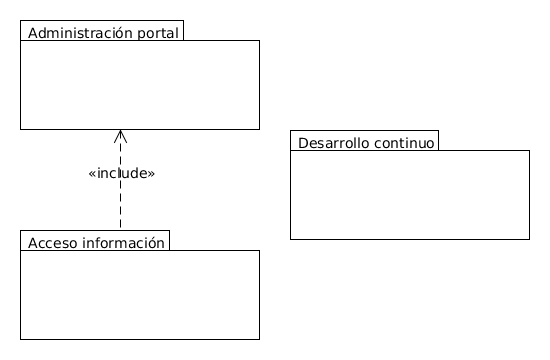
\includegraphics[width=0.8\textwidth]{imagenes/diagrama_paquetes.png}
  \caption{Diagrama de paquetes}
  \label{fig:diag_paquetes}
  \end{center}
\end{figure}
 
\section{Diagramas de casos de uso}

\begin{figure}[!ht]
  \begin{center}
  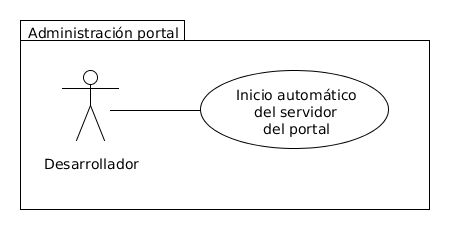
\includegraphics[width=0.65\textwidth]{imagenes/diag_cu_ap.png}
  \caption{Diagrama de casos de uso: paquete Administración portal}
  \label{fig:diag_cu_ap}
  \end{center}
\end{figure}

\begin{figure}[!ht]
  \begin{center}
  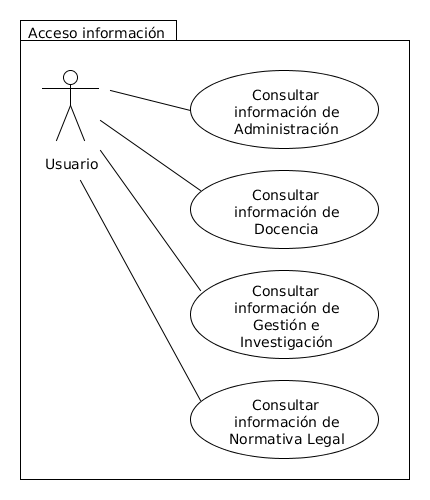
\includegraphics[width=0.65\textwidth]{imagenes/diag_cu_ai.png}
  \caption{Diagrama de casos de uso: paquete Acceso información}
  \label{fig:diag_cu_ai}
  \end{center}
\end{figure}

\begin{figure}[!ht]
  \begin{center}
  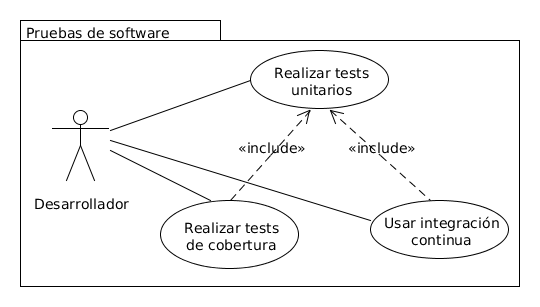
\includegraphics[width=0.65\textwidth]{imagenes/diag_cu_ps.png}
  \caption{Diagrama de casos de uso: paquete Pruebas de software}
  \label{fig:diag_cu_ps}
  \end{center}
\end{figure}

\begin{figure}[!ht]
  \begin{center}
  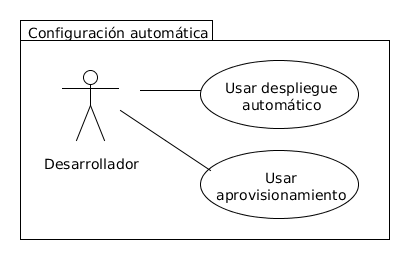
\includegraphics[width=0.65\textwidth]{imagenes/diag_cu_ca.png}
  \caption{Diagrama de casos de uso: paquete Configuración automática}
  \label{fig:diag_cu_ca}
  \end{center}
\end{figure}

\newpage
\
\newpage
\section{Diagramas de actividad}

\begin{figure}[!ht]
  \begin{center}
  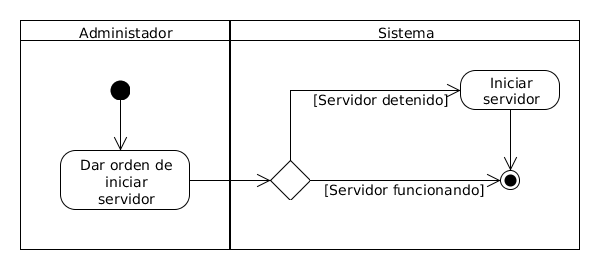
\includegraphics[width=1\textwidth]{imagenes/diag_act_cu_01.png}
  \caption{Diagrama de actividad CU-1. Inicio automático del servidor del portal}
  \label{fig:diag_act_cu_01}
  \end{center}
\end{figure}

\begin{figure}[!ht]
  \begin{center}
  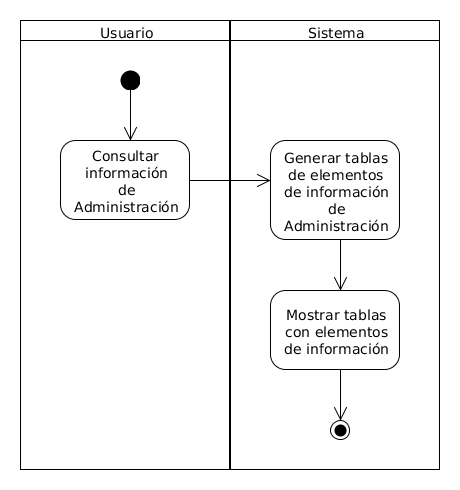
\includegraphics[width=1\textwidth]{imagenes/diag_act_cu_02.png}
  \caption{Diagrama de actividad CU-2. Consultar información de Administración}
  \label{fig:diag_act_cu_02}
  \end{center}
\end{figure}

\begin{figure}[!ht]
  \begin{center}
  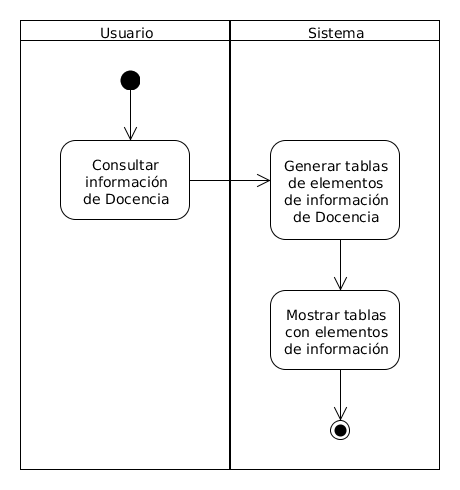
\includegraphics[width=1\textwidth]{imagenes/diag_act_cu_03.png}
  \caption{Diagrama de actividad CU-3. Consultar información de Docencia}
  \label{fig:diag_act_cu_03}
  \end{center}
\end{figure}

\begin{figure}[!ht]
  \begin{center}
  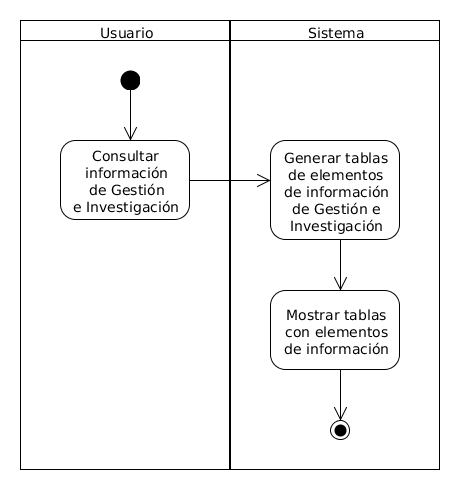
\includegraphics[width=1\textwidth]{imagenes/diag_act_cu_04.png}
  \caption{Diagrama de actividad CU-4. Consultar información de Gestión e Investigación}
  \label{fig:diag_act_cu_04}
  \end{center}
\end{figure}

\begin{figure}[!ht]
  \begin{center}
  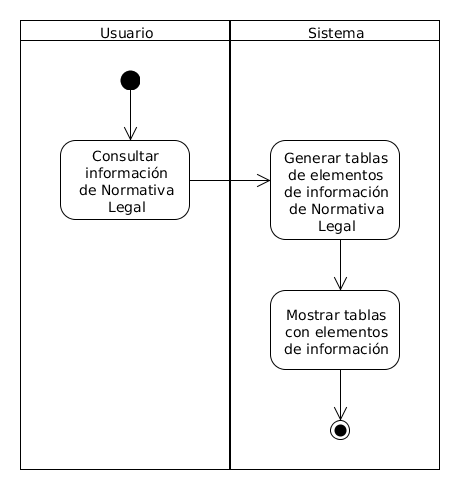
\includegraphics[width=1\textwidth]{imagenes/diag_act_cu_05.png}
  \caption{Diagrama de actividad CU-5. Consultar información de Normativa Legal}
  \label{fig:diag_act_cu_05}
  \end{center}
\end{figure}

\begin{figure}[!ht]
  \begin{center}
  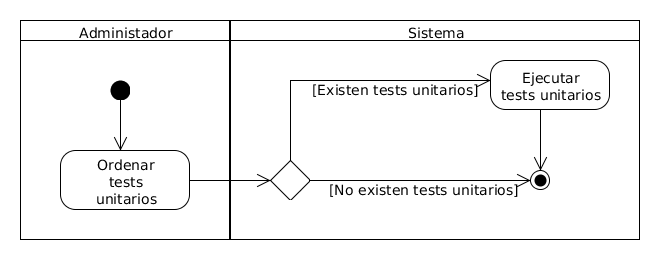
\includegraphics[width=1\textwidth]{imagenes/diag_act_cu_06.png}
  \caption{Diagrama de actividad CU-6. Realizar tests unitarios}
  \label{fig:diag_act_cu_06}
  \end{center}
\end{figure}

\begin{figure}[!ht]
  \begin{center}
  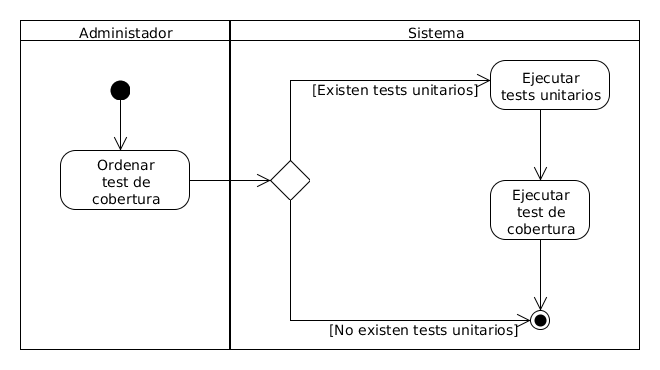
\includegraphics[width=1\textwidth]{imagenes/diag_act_cu_07.png}
  \caption{Diagrama de actividad CU-7. Realizar test de cobertura}
  \label{fig:diag_act_cu_07}
  \end{center}
\end{figure}

\begin{figure}[!ht]
  \begin{center}
  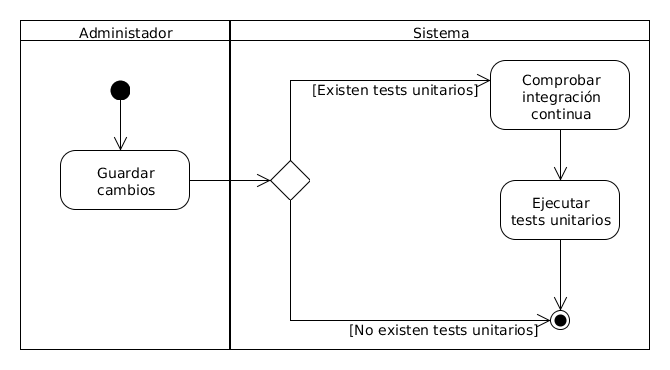
\includegraphics[width=1\textwidth]{imagenes/diag_act_cu_08.png}
  \caption{Diagrama de actividad CU-8. Usar integración continua}
  \label{fig:diag_act_cu_08}
  \end{center}
\end{figure}

\begin{figure}[!ht]
  \begin{center}
  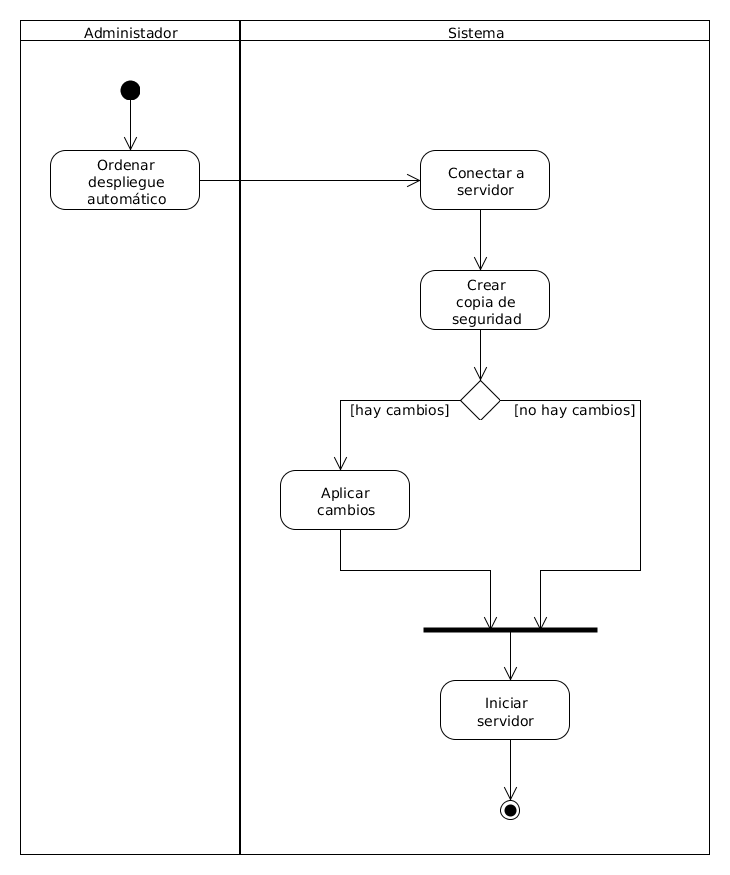
\includegraphics[width=1\textwidth]{imagenes/diag_act_cu_09.png}
  \caption{Diagrama de actividad CU-9. Usar despliegue automático}
  \label{fig:diag_act_cu_09}
  \end{center}
\end{figure}

\begin{figure}[!ht]
  \begin{center}
  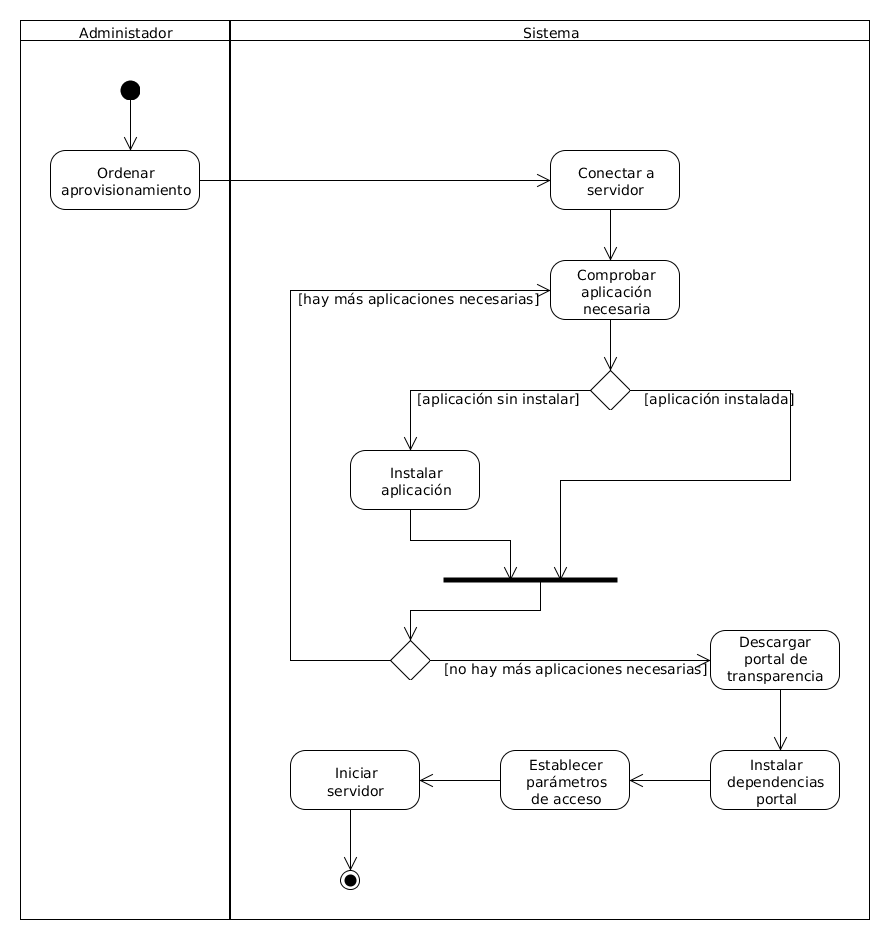
\includegraphics[width=1\textwidth]{imagenes/diag_act_cu_10.png}
  \caption{Diagrama de actividad CU-10. Usar aprovisionamiento}
  \label{fig:diag_act_cu_10}
  \end{center}
\end{figure}

\newpage
\
\newpage
\
\newpage
\
\newpage
\
\newpage
\
\newpage
\
\newpage
\
\newpage
\
\newpage

\section{Diagrama conceptual}

\begin{figure}[!ht]
  \begin{center}
  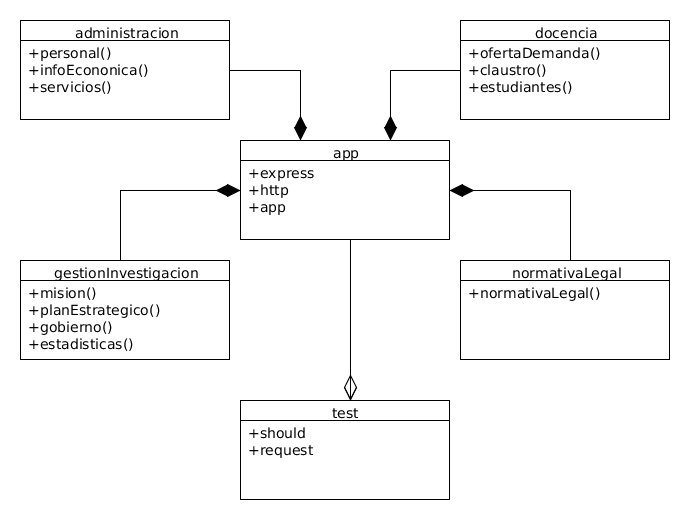
\includegraphics[width=1\textwidth]{imagenes/diagrama_conceptual.png}
  \caption{Diagrama conceptual}
  \label{fig:diagrama_conceptual}
  \end{center}
\end{figure}
%
%\chapter{Diseño}

\section{Diseño general del portal}

Para describir el diseño que se va a seguir en la programación del proyecto hay que tener en cuenta que se va a usar {\tt Node.js}, que está basado en el lenguaje de programación {\tt JavaScript} (que es un lenguaje orientado a objetos). Se usará un paradigma de programación orientado a objetos con diversas clases, que en este entorno de programación suelen ser referidos como módulos.

\bigskip
Existirá un módulo principal de la plataforma ({\tt app.js}) que será la plataforma en si misma, que es el encargado de generar el servidor al que se realizarán las peticiones y visualizar cada unas de las páginas. Existirán también un módulo por cada una de las secciones del portal: Administración ({\tt administración.js}), Docencia ({\tt docencia.js}), Gestión e Investigación ({\tt gestionInvestigación.js}) y Normativa Legal ({\tt normativaLegal.js}. Si comparamos este esquema con el de una aplicación más tradicional, podríamos considerar el módulo ({\tt app.js}) como la clase principal y el resto de módulos como otras clases que tienen como función ser atributos compuestos de esa clase principal.

\bigskip
Cada uno de estos módulos de las diversas secciones, obtendrá la información para generar las páginas de sus subsecciones desde un archivo de datos {\tt JSON}, organizados de la siguiente forma.

\newpage
\begin{itemize}
 \item UGR Transparente ({\tt app.js}).
 \begin{itemize}
  \item Administración ({\tt administración.js}).
  \begin{itemize}
   \item Personal ({\tt personal.json}).
   \item Información Económica ({\tt infoEcononica.json}).
   \item Servicios ({\tt servicios.json}).
  \end{itemize}
  \item Docencia.
  \begin{itemize}
   \item Oferta y Demanda Académica ({\tt ofertaDemanda.json}).
   \item Claustro ({\tt claustro.json}).
   \item Estudiantes ({\tt estudiantes.json}).
  \end{itemize}
  \item Gestión e Investigación.
  \begin{itemize}
   \item Misión ({\tt mision.json}).
   \item Plan Estratégico ({\tt .json}).
   \item Gobierno ({\tt gobierno.json}).
   \item Estadísticas ({\tt estadistica.json}).
  \end{itemize}
  \item Normativa Legal.
  \begin{itemize}
   \item Normativa Legal ({\tt normativaLegal.json}).
  \end{itemize}
 \end{itemize}
\end{itemize}

Cada vez que un usuario quiere consultar la información de una subsección, el portal de transparencia (UGR Transparente) hace una llamada al método de generación de la página de la sección elegida para su subsección determinada; ese método, procesará la plantilla {\tt Jade} para la página pasándole el archivo {\tt JSON} de datos y el resultado final será la página web que será visible en el portal.

\bigskip
De igual forma a lo mencionado de la aplicación del portal de transparencia, los test unitarios ({\tt test.js}) y el despliegue automático ({\tt flightplan.js}) son otros módulos que ejecutan dichas acciones, el test de cobertura se realiza automáticamente a partir de los test unitarios, la integración continua se realiza en base a la configuración del archivo {\tt .travis.yml}, y finalmente, el aprovisionamiento sigue las tareas en el archivo de configuración {\tt transparente.yml}. Todos estos módulos son independientes del funcionamiento del módulo principal, y simplemente llamaremos cuando queramos hacer uso de sus funcionalidades.

\newpage
\section{Diseño de una aplicación con desarrollo colaborativo}

En varias ocasiones se ha indicado que este proyecto parte de un desarrollo colaborativo, esto es debido a que hoy en día es muy difícil concebir un proyecto de software libre fuera de un entorno colaborativo que permita publicar el código libremente en Internet donde sea accesible por cualquier persona, esta filosofía es la que sigue por ejemplo el desarrollo de {\tt Linux} a principio de los años 90, el que se podría considerar como el más grande y relevante proyecto de software libre a nivel mundial. Además de abogar por la transparencia, este sistema de desarrollo hace que se más fácil encontrar errores durante el desarrollo ya que un mayor número de personas tienen acceso total al mismo. También hay que tener en cuenta como en todo proyecto que es imprescindible una herramienta de control de versiones, aún más en uno colaborativo donde es fácil que se produzcan conflictos en los archivos modificados por unos y otros desarrolladores.

\bigskip
La plataforma de desarrollo colaborativo y la herramienta de control de versiones a usar son {\tt GitHub} y {\tt Git} respectivamente. {\tt GitHub} es una de las plataformas de desarrollo colaborativo más usadas en proyectos libres y usa {\tt Git} como sistema de control de versiones para gestionar los proyectos que se almacenan en la plataforma. Estás son las herramientas que nos van a permitir que nuestro proyecto se convierta en un proyecto que se desarrollo de forma ágil,  concretamente se va a seguir una metodología {\tt DevOps}.

\bigskip
Una metodología de desarrollo {\tt DevOps} consiste inicialmente en no hacer distinción entre el desarrollo del software y la administración del mismo, todo estará comunicado para que sea posible realizar entregas del software de forma frecuente asegurándose de que esas mismas entregas continuas no sea el origen de fallos futuros. La forma de asegurarse de que esos fallos no se producirán es dividir todo el desarrollo en fases que tengan que realizarse secuencialmente, controlando a cada fase que no se produzcan errores en la misma; como una cadena de montaje en la que podemos estar seguro de que el producto que llega al final está en perfectas condiciones, porque en caso contrario hubiera sido retirado durante el proceso.

\bigskip
En este proyecto, hemos considerado que las fases que nos permitirían asegurarnos que el producto que sale de la cadena de montaje en perfectas condiciones sean los test unitarios, la integración continua y el despliegue automático, todo esto apoyado en un sistema de control de versiones y una plataforma de desarrollo colaborativo abierto. Además, también se usará aprovisionamiento para facilitar la portabilidad del portal de una infraestructura a otra distinta. 

\section{Diseño de los tests unitarios y test de cobertura}

Para cumplir la parte de testeo de la implementación de la metodología {\tt DevOps}, a partir del desarrollo de este proyecto se pretende seguir un desarrollo guiado por pruebas (en inglés, {\tt Test-Driven Development} o {\tt TDD}). Esto consiste en escribir primero las pruebas que consideremos que la aplicación debe superar y luego desarrollar el código que realice la función que queremos cumplir, pero superando dichas pruebas. 

\bigskip
Estas pruebas estarán basadas en la ejecución de tests unitarios que estarán diseñados para comprobar de forma de automática que el código escrito cumple con el objetivo determinado; por lo que si una vez ejecutamos todos los tests unitarios, si no obtenemos que todos han tenido una ejecución exitosa, tenemos que revisar el código escrito para saber por qué fallan.

\bigskip
Haciendo esto nos aseguraremos que todos las funcionalidades que vayamos añadiendo a la implementación de la aplicación funcionarán correctamente; también nos asegura que si tenemos que hacer grandes modificaciones en el código, siempre que estas modificaciones sigan pasando las pruebas, no deberemos preocuparnos por estropear el funcionamiento de la aplicación.

\bigskip
El tipo de test unitario que vamos a usar es un test basado en el comportamiento, es decir, la forma de evaluar si un test se supera con éxito o fracaso es mediante la comprobación de la respuesta que da nuestra aplicación ante una solicitud 
determinada. Ejemplos:

\begin{itemize}
 \item Para comprobar que un archivo con datos de configuración ha sido cargado, el archivo cargado no debe ser nulo.
 \item Para comprobar que en la información cargado se encuentra el nombre de la categoría, la categoría debe tener una propiedad llamada ``nombre''.
 \item Para comprobar que las páginas del portal están accesibles, las respuesta a las solicitudes se espera que tenga el valor 200 (código de respuesta estándar para peticiones correctas en conexiones {\tt HTTP}).
\end{itemize}

Pero el diseño de las pruebas no termina con escribir los tests unitarios que consideremos oportunos, también es necesario que esos tests pasen a su vez un test de cobertura. Un test de cobertura comprueba el porcentaje de código desarrollado y/o número de funciones de la aplicación que se están evaluando con los tests unitarios desarrollados, con esto se puede verificar la completitud de los tests unitarios; si todos nuestros tests unitarios se evalúan correctamente, pero solo están cubriendo un 30\% del total de la aplicación, este resultado satisfactorio no nos puede asegurar que la funcionalidad completa de la aplicación se vaya a ejecutar sin problemas.

\bigskip
Los tests unitarios se van a desarrollar usando {\tt Should} y {\tt Supertest}, ambos módulos de {\tt Node.js} para evaluar comportamientos en las peticiones. Estos tests unitarios a su vez van a ser evaluados por {\tt Mocha}, un framework de {\tt JavaScript} para testeo que se ejecuta tanto en aplicaciones {\tt Node.js} como en navegadores web. Por último, todo esto pasará por las pruebas de cobertura de código de {\tt Istanbul}, que generará un informa detallado especificando la cantidad de código y el número de funciones que están cubiertas y también los que no.

\section{Diseño de la integración continua}

La integración continua (en inglés, \textit{continuous integration} o {\tt CI}) consiste en comprobar cada vez que hacemos cambios en el código de la aplicación esto no genere problemas en su ejecución, ya que el cambio del comportamiento en una simple función puede cambiar en gran parte el comportamiento de la aplicación entera, y si otra función requiere del resultado de esta última, las consecuencias pueden ser desastrosas. Teniendo en cuenta que vamos a trabajar en un entorno de desarrollo colaborativo, es todavía más necesario que se asegure la integridad de la aplicación frente a los cambios.

\bigskip
Para que esto se pueda realizar, con cada cambios se activará automáticamente un proceso que verificará mediante la ejecución de los tests unitarios escritos que los cambios realizados no producen errores en la aplicación. Al igual que pasaba con los tests unitarios, la integración continua es una medida que nos permite incrementar la calidad del software producido porque cuanto más a menudo se hagan estas comprobaciones, mayor será la facilidad para detectar fallos en el propio software.

\bigskip
Realizaremos la integración continua a través de {\tt Travis CI}, que es un sistema distribuido de integración continua libre que está integrado con {\tt GitHub}. Este sistema además tiene como ventajas el soporte para numerosos lenguajes y la posibilidad de ejecutar las pruebas en distintas versiones del propio lenguaje, por lo que fácilmente podríamos probar nuestro desarrollo con diferentes configuraciones sin tener que realizar cambios en nuestro sistema local.

\bigskip
El procedimiento para realizar la integración continua consistirá en configurar el repositorio del proyecto en {\tt GitHub} para que cada vez se realice un cambio en los archivos del repositorio, este iniciará un proceso por el cual se creará un \textit{build} automático en un servidor virtual de {\tt Travis CI} que se ha creado con tal finalidad y se desplegará en él la última versión con los cambios que acabamos de realizar, para acto seguido ejecutar las pruebas que hayamos desarrollado y generar un informe sobre los resultados de las pruebas para cada una de las configuraciones que hayamos definido para la integración continua. Estos informes son almacenados en el propio sitio de {\tt Travis}, recibiendo un aviso por correo en el caso de que las pruebas no hayan finalizado exitosamente en alguna de las configuraciones.

\section{Diseño del despliegue automático}

Una vez que tenemos la seguridad de que toda la aplicación funciona correctamente, solo nos queda desplegarla en nuestro servidor de producción; además, vamos a automatizar las tareas que deberíamos realizar manualmente para evitar posibles errores. En esto consiste el despliegue automático, hacer efectivos los cambios en nuestro software de nuestro software en una o varias plataformas objetivo sin que tengamos que realizar personalmente y paso a paso el proceso necesario para ello, todo es 
automatizado.

\bigskip
Antes de pasar a implementar el despliegue automático, hay que pensar que tareas es necesario o queremos que se realicen. Independientemente del tipo de aplicación, como medida preventiva se debe hacer una copia de seguridad del estado actual de la aplicación desplegada en el servidor. La ejecución del portal depende de que el servidor creado por {\tt Express} esté en  ejecución, por lo que antes de desplegar la nueva versión, se debería detener la ejecución de la versión anterior. Con todo esto hecho solo nos quedaría obtener los propios cambios realizamos, comprobar que todas las dependencias se siguen cumpliendo y  establecer los parámetros para que el servidor sea accesible desde {\tt Internet}; para finalizar la tarea, se iniciaría la ejecución de la aplicación.

\bigskip
Todas las tareas descritas, queremos que sean ejecutadas de forma secuencial una tras otra, de forma automática y necesitar la interacción con el usuario. Para cumplir esto usaremos {\tt Flightplan}, un módulo de {\tt Node.js} que nos permite coordinar de forma automática el despliegue de aplicaciones con tareas de administración del sistema.

\newpage
\section{Diseño del aprovisionamiento}

Con toda la aplicación ya realizada, para su instalación inicial en un plataforma determinada primero tenemos que aprovisionarla con todos los recursos software necesarios. Encontraremos una mayor cantidad de referencias a este procedimiento por su término en ingles, software provisioning, ya que el termino en español es una traducción literal que salvo por el acompañamiento del termino \textit{``software"}, puede referirse a abastecimientos de recursos necesarios en general no necesariamente relacionado con el campo de la informática.

\bigskip
Entre el software básico necesario hay que considerar para instalar la propia plataforma del desarrollo de la aplicación ({\tt Node.js}) y la herramienta de control de versiones ({\tt Git}). Con esto instalado, se clona el repositorio en {\tt GitHub} del proyecto en un directorio local, y una vez instalada las dependencias de la aplicación y establecidos los parámetros de acceso, se arrancará el servidor para que el portal esté funcionando.

\bigskip
Todas estas tareas se harán de forma automática, para ello usaremos {\tt Ansible}, una aplicación de software libre que nos permitirá configurar y administrar los ordenadores que indiquemos en la lista de hosts objetivo. Su funcionamiento básicamente se basa en conectarse al ordenador a configurar mediante una conexión {\tt SSH} (por lo que deberemos indicarle con el usuario que tiene que realizarse la conexión) e irá ejecutando secuencialmente cada unas de las tareas del archivo {\tt YAML} de su archivo de configuración (al que se hace referencia como \textit{playbook}).
%
%\chapter{Implementación}

Partiendo del trabajo previo...

\section{Uso de JSON como origen de datos}

\section{Tests unitarios y de cobertura}

\section{Integración continua}

\section{Despliegue automático}

\section{Aprovisionamiento}
%
%\chapter{Pruebas}

En el capítulo anterior se describía como se había realizado toda la implementación del proyecto, por lo que ya solo queda probar que todo funciona correctamente.

\section{Pruebas unitarias}

Para ejecutar las pruebas unitarias vamos a ejecutar con {\tt Mocha} a través de {\tt Istanbul}, realizando las pruebas unitarias y generando el resultado de la prueba de cobertura en un misma ejecución. Cuando ejecutemos {\tt npm test} comenzarán a comprobarse una por una todas las comprobaciones en el archivo {\tt tests.js}; las llamadas al método {\tt describe} son las líneas que aparecen como título en blanco mientras que las comprobaciones que se hacían con el método {\tt it} son las líneas en gris, que aparecen con un \textit{check} verde si el valor esperado es el correcto ó, en caso de error, con un número rojo que indique el error de forma enumerada.

\bigskip
Una vez que todas las comprobaciones hayan sido realizadas nos aparecerá un resumen con los resultados de los test pasados, indicando cuantos se han ejecutado correctamente (\textbf{passing}) y cuantos han producido un error (\textbf{failing}); si alguna de las tareas asíncronas no devolviera el mensaje {\tt done} estas quedarían como comprobaciones pendientes (\textbf{pending}), pero esto es algo que no se produce en nuestro caso.

\begin{figure}[!ht]
	\begin{center}
		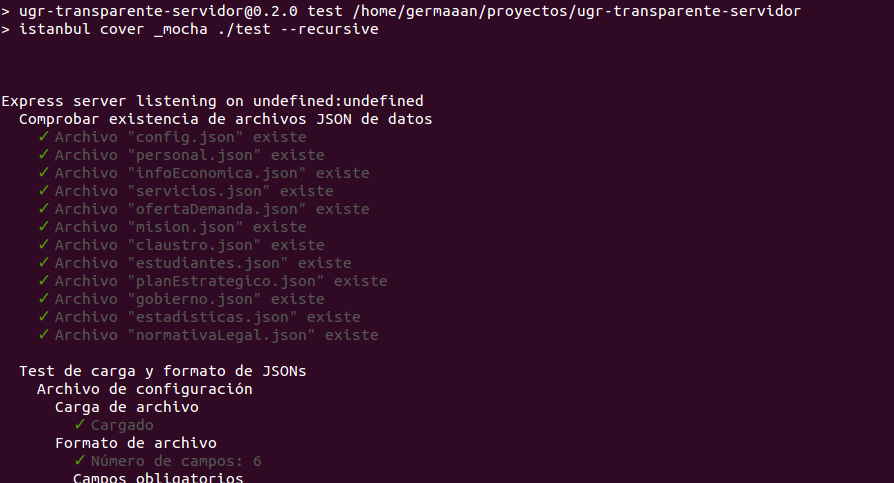
\includegraphics[width=1\textwidth]{../images/tests_unitarios_01.png}
		\caption{Ejecución de los test unitarios con Mocha (1/2)}
		\label{fig:tests_unitarios_01}
	\end{center}
\end{figure}

\newpage
En la siguiente imagen vemos que todas los tests se han pasado correctamente (\textbf{148 passing}) en un tiempo de \textbf{3 segundos}. Además, como hemos dicho que {\tt Mocha} es ejecutado a través de {\tt Istanbul}, también obtenemos el mensaje de que el test de cobertura se ha generado dentro de la carpeta {\tt coverage} y un resumen de la cobertura del código que realizan nuestros test.

\begin{figure}[!ht]
	\begin{center}
		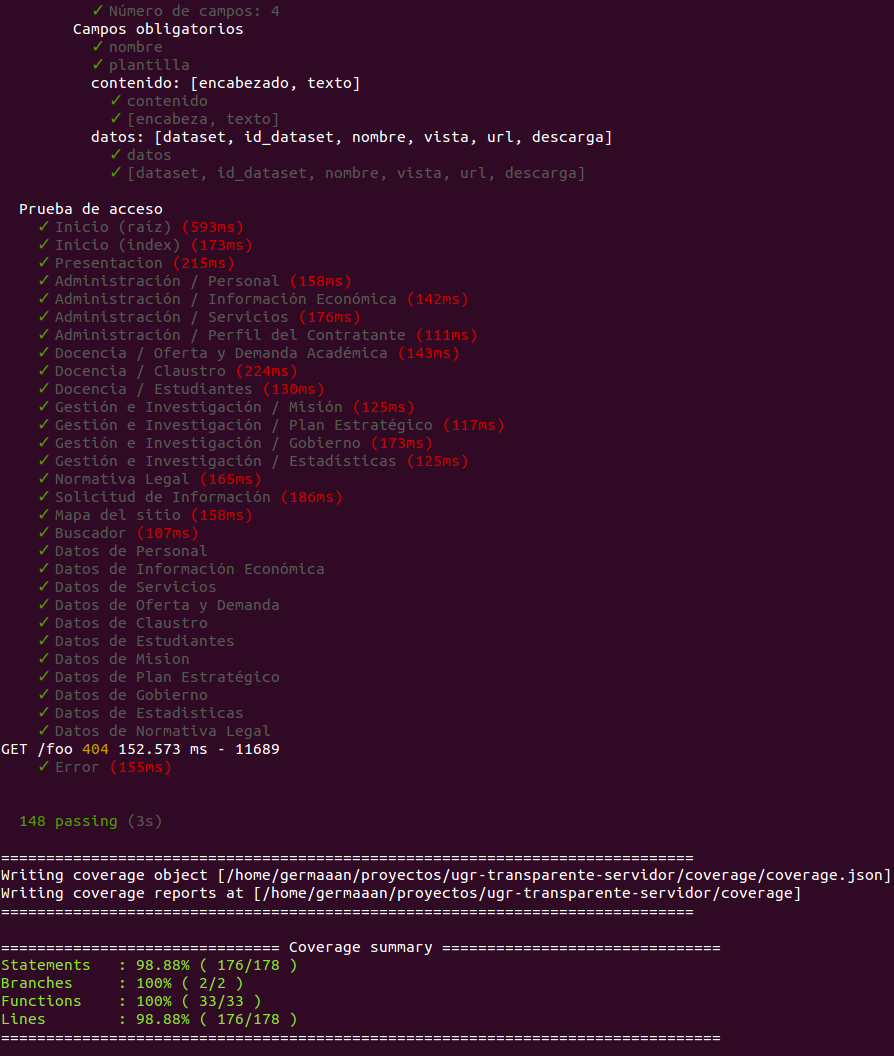
\includegraphics[width=1\textwidth]{../images/tests_unitarios_02.png}
		\caption{Ejecución de los test unitarios con Mocha (2/2)}
		\label{fig:tests_unitarios_02}
	\end{center}
\end{figure}

\newpage
Si alguno de los test fallara (por ejemplo, uno de los archivos de origen de datos no existe) en el resumen además del número de test fallados, se mostrará una descripción de los mismos. Es el caso de la siguiente imagen, el archivo {\tt personal.json} no existe por lo que entre los 11 errores que se han producido vemos que en la comprobación de la existencia del archivo se produce un aserción debido a que el resultado esperado por {\tt Mocha} es \textbf{true} y sin embargo recibe \textbf{false} en su lugar}, relacionado con esto nos encontramos el siguiente error y es que como no se ha podido cargar el archivo no se han podido comprobar las propiedades que deberían tener ese archivo (la propiedad que espera \textbf{should} es nula).

\begin{figure}[!ht]
	\begin{center}
		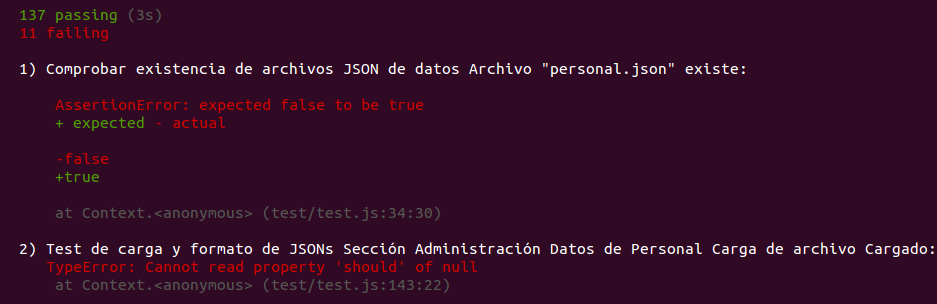
\includegraphics[width=1\textwidth]{../images/tests_unitarios_03.png}
		\caption{Error en tests unitarios}
		\label{fig:tests_unitarios_03}
	\end{center}
\end{figure}

\section{Prueba de cobertura}

Como veíamos al finalizar los test unitarios, el resultado del test de cobertura se almacena en la carpeta {\tt coverage}, dentro de dicha carpeta encontraremos un archivo \textit{HTML} con el mismo resumen que aparecía al finalizar la ejecución de los tests unitarios, pero en este caso permitiéndonos acceder a una información más completa. 

\begin{figure}[!ht]
	\begin{center}
		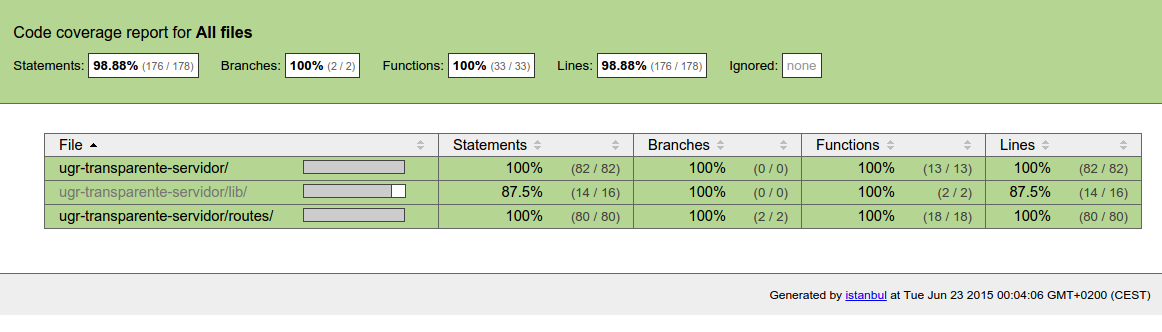
\includegraphics[width=1\textwidth]{../images/test_cobertura_01.png}
		\caption{Resumen de resultados de test de cobertura}
		\label{fig:test_cobertura_01}
	\end{center}
\end{figure}

Por ejemplo, vamos a comprobar más detalladamente la cobertura en el código de la aplicación principal de la plataforma, por lo que seleccionamos \textbf{ugr-transparente-servidor} y después el archivo de nuestra aplicación {\tt app.js}. En el resumen todo el código de esta parte de la aplicación aparecía con una cobertura del \textbf{100\%} por eso todas las líneas del código aparecen en verde.

\begin{figure}[!ht]
	\begin{center}
		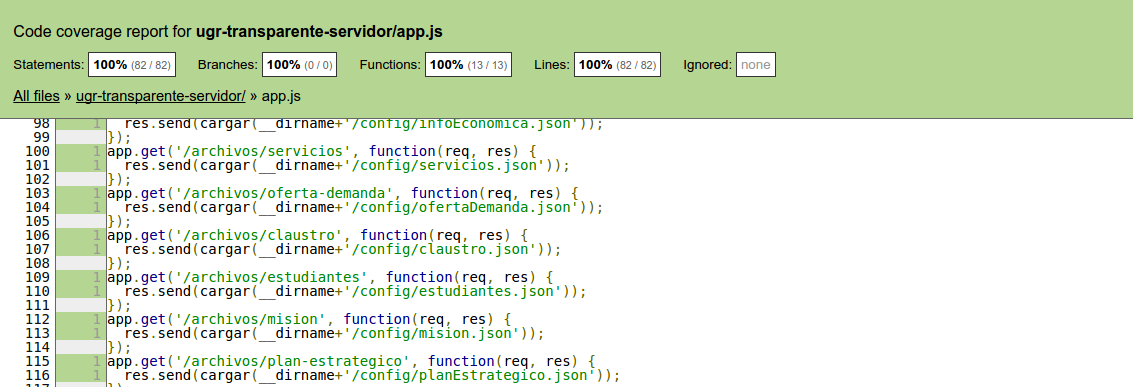
\includegraphics[width=1\textwidth]{../images/test_cobertura_02.png}
		\caption{Resultado de cobertura de la aplicación principal}
		\label{fig:test_cobertura_02}
	\end{center}
\end{figure}

En el caso de que alguna sentencia no estuviera cubierta por los test unitarios, esta aparecería en rojo; esto es lo que sucede por ejemplo en uno de los módulos desarrollado: cuando se captura una excepción espera que sea lanzadaa a un nivel superior sin embargo solo se muestra un mensaje por pantalla, {\tt Istanbul} aprecia esto como un fallo de cobertura y por eso destaca esa línea en rojo.

\begin{figure}[!ht]
	\begin{center}
		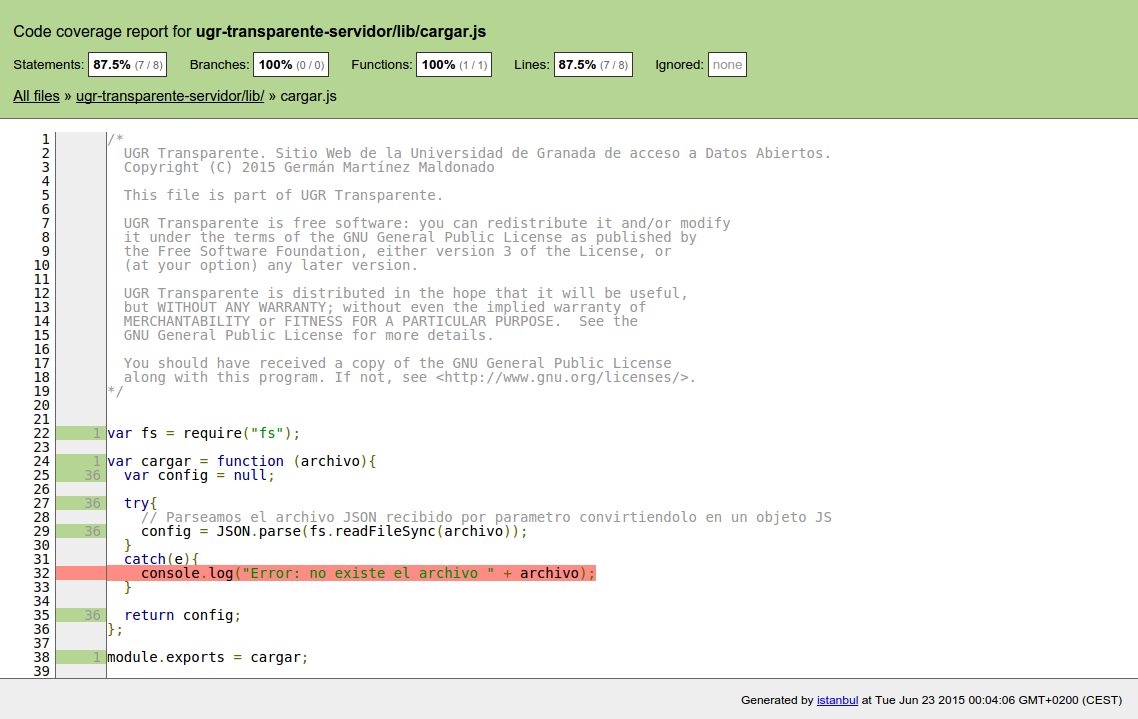
\includegraphics[width=1\textwidth]{../images/test_cobertura_03.png}
		\caption{Resultado de cobertura de un módulo desarrollado}
		\label{fig:test_cobertura_03}
	\end{center}
\end{figure}

\newpage
\section{Integración continua}

Tenemos los test unitarios hecho y hemos comprobado que funcionan, por lo que teniendo la configuración de {\tt Travis CI} realizada, cada vez que se haga un \textit{push} al repositorio se generará un \textit{build} en sus servidores para comprobar que los nuevos cambios introducidos no producen errores en la aplicación. Esta comprobación se hará en cada una de las versiones de nuestro lenguaje que hayamos definido, obteniendo un resumen al final de su ejecución que nos indicará si todo se ha ejecutado correctamente; dicho resultado es accesible a través de su página web (\url{https://travis-ci.org/oslugr/ugr-transparente-servidor}). En la imagen siguiente tenemos el resultado de un \textit{build} en el que no se ha producido ningún error, por lo que todos pruebas de las diferentes versiones están marcadas con un \textit{check} verde.

\begin{figure}[!ht]
	\begin{center}
		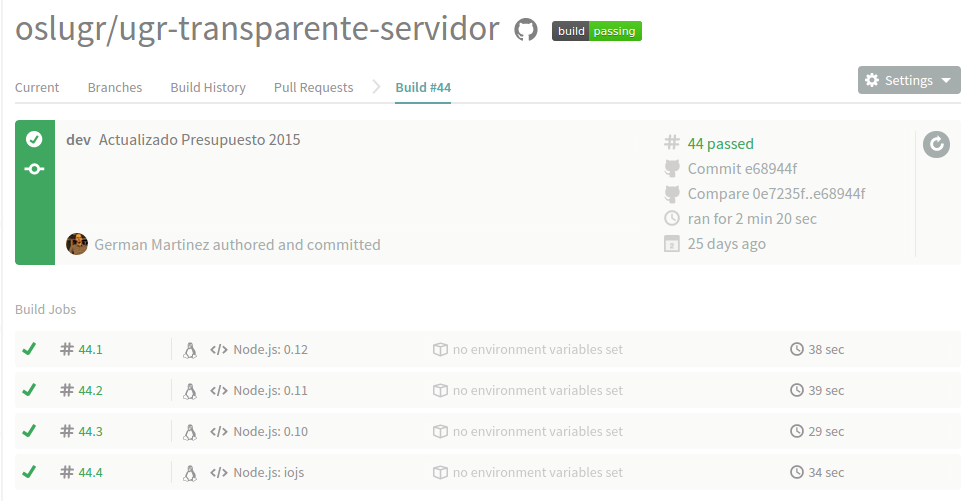
\includegraphics[width=1\textwidth]{../images/integracion_continua_01.png}
		\caption{}
		\label{fig:integracion_continua_01}
	\end{center}
\end{figure}

Si seleccionamos en concreto alguna de las entradas, obtendremos la salida del despliegue de la aplicación y la posterior ejecución de los test.

\begin{figure}[!ht]
	\begin{center}
		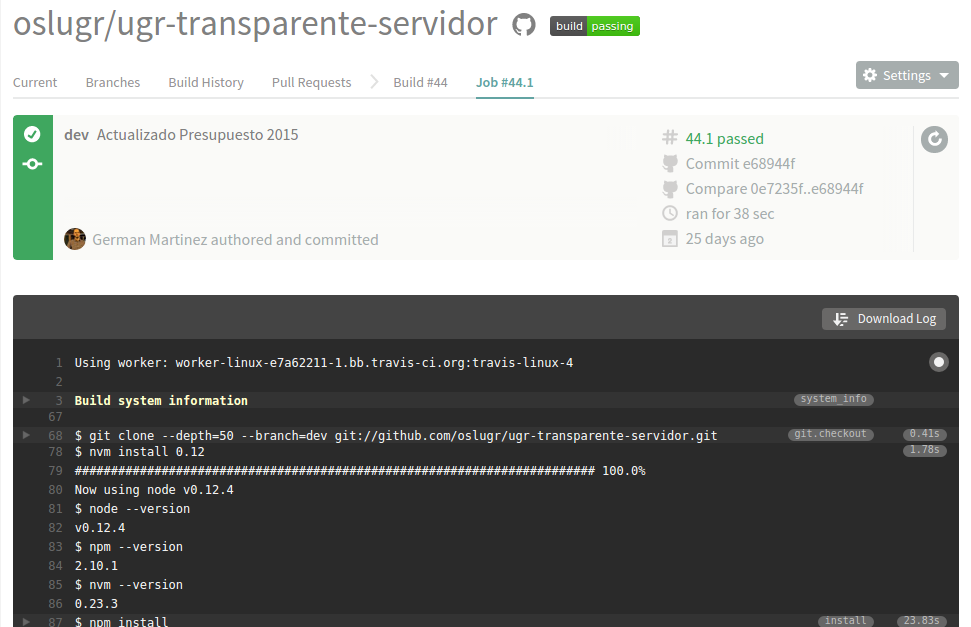
\includegraphics[width=1\textwidth]{../images/integracion_continua_02.png}
		\caption{Salida del build en Travis CI (despliegue)}
		\label{fig:integracion_continua_02}
	\end{center}
\end{figure}

La salida de la ejecución de los tests es exactamente igual a la salida que hemos visto que se produce se ejecutamos los tests de forma local llamando a {\tt npm test} (que es lo hace {\tt Travis} igualmente).

\begin{figure}[!ht]
	\begin{center}
		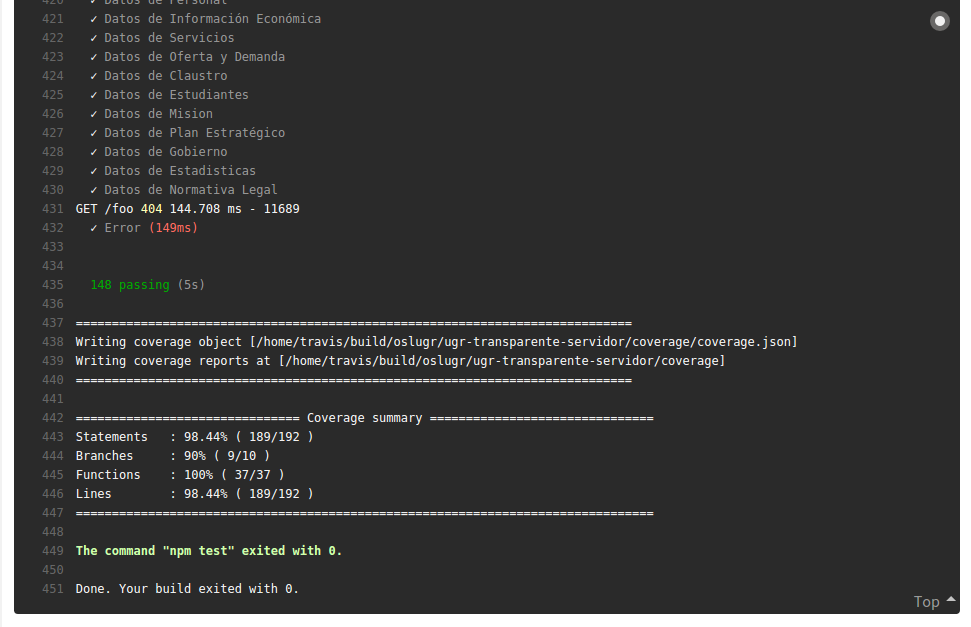
\includegraphics[width=1\textwidth]{../images/integracion_continua_03.png}
		\caption{Salida del build en Travis CI (resultados tests)}
		\label{fig:integracion_continua_03}
	\end{center}
\end{figure}

\section{Despliegue automático}

También vamos a comprobar que el despliegue automático funciona correctamente. Simplemente ejecutamos el script {\tt deploy} pasándole como parámetro el usuario con el que nos conectaremos al servidor. En la imagen siguiente vemos el resultado de la ejecución, aunque no en este momento no había nuevos cambios que aplicar al servidor, si podemos ver como hace la copia de seguridad inicial y ejecuta el resto de órdenes necesarias para que la aplicación del portal quede en funcionamiento.

\begin{figure}[!ht]
	\begin{center}
		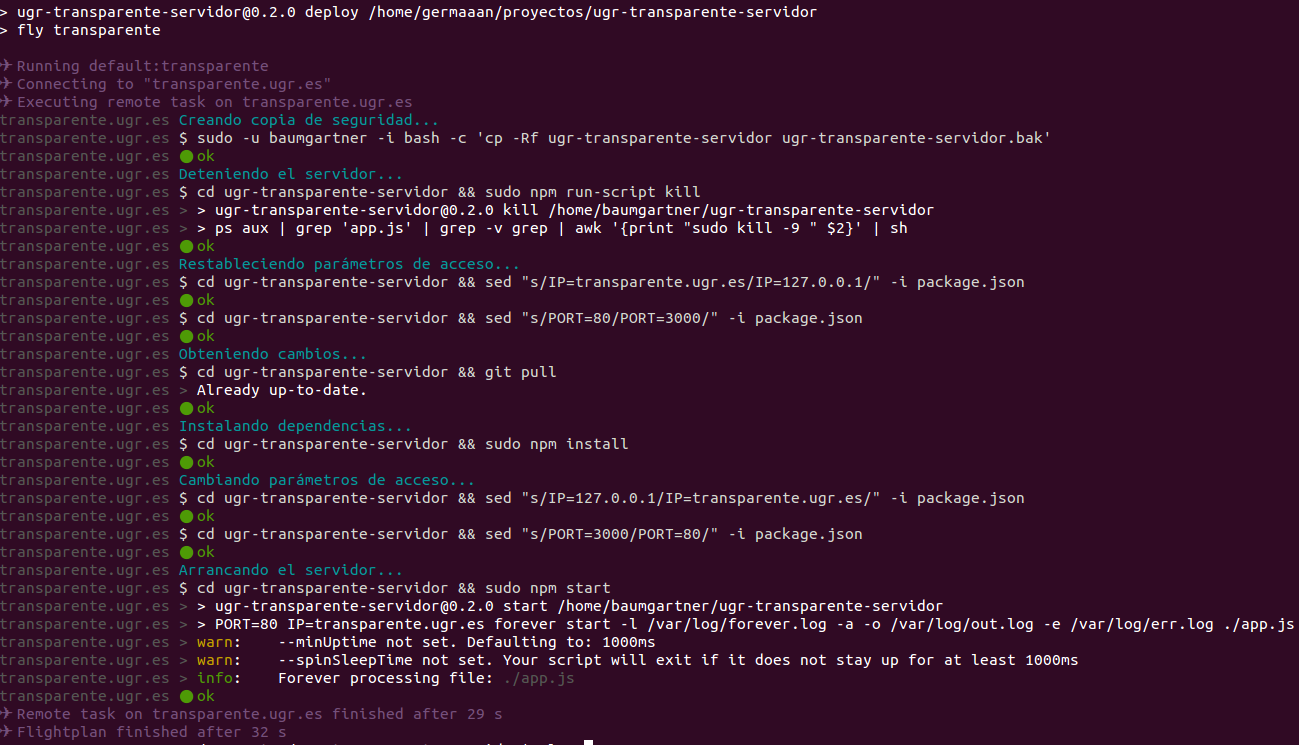
\includegraphics[width=1\textwidth]{../images/deploy.png}
		\caption{Ejecución de despliegue automático}
		\label{fig:deploy}
	\end{center}
\end{figure}

\newpage
\section{Aprovisionamiento}

Como el sitio de {\tt UGR Transparente} está funcionando sin problemas en este momento, para probar el aprovisionamiento crearemos una máquina virtual con {\tt Vagrant} con el mismo sistema operativo que se encuentra en el servidor de la plataforma ({\tt Ubuntu 14.04}) para realizarle el aprovisionamiento con el {\tt playbook} escrito para {\tt Ansible}.

\bigskip
Las órdenes a introducir para crear la máquina virtual son las que aparecen en el siguiente fragmento de código.

\begin{lstlisting}[language=bash,captionpos=b,caption={Órdenes para crear máquina virtual Vagrant},label={lst:crear_vagrant}]
vagrant box add ubuntu/trusty64
vagrant init ubuntu/trusty64
vagrant up
vagrant ssh
\end{lstlisting}

\newpage
También tenemos que crear un archivo {\tt Vagrantfile} en el que es importante establecer la dirección de acceso a la máquina y como provisionador {\tt Ansible}, indicando también el \textit{playbook} que se va a utilizar.

\begin{lstlisting}[language=Ruby,captionpos=b,caption={Archivo Vagrantfile},label={lst:edit_vgfile}]
# -*- mode: ruby -*-
# vi: set ft=ruby :

VAGRANTFILE_API_VERSION = "2"

Vagrant.configure(VAGRANTFILE_API_VERSION) do |config|
	config.vm.box = "ubuntu/trusty64"
	config.vm.network :private_network, ip:"192.168.2.50"

	config.vm.provision "ansible" do |ansible|
		ansible.playbook = "transparente.yml"
	end
end
\end{lstlisting}

Lo siguiente será cambiar en el archivo {\tt ansible\_hosts} la dirección del portal por la dirección de nuestra máquina virtual (comando {\tt sed}), declarar como variable de entorno archivo {\tt ansible\_hosts} (comando {\tt export}), y finalmente con {\tt Vagrant}, recargar la configuración del {\tt Vagrantfile} ({\tt vagrant reload}) y ordenar el aprovisionamiento de la máquina virtual ({\tt vagrant provision}). En el siguiente fragmento de código se listan todos estos comandos y en la imagen que le sigue se puede comprobar la ejecución, obteniendo como resultado un aprovisionamiento completamente exitoso.

\begin{lstlisting}[language=bash,captionpos=b,caption={Órdenes para aprovisionar máquina Vagrant},label={lst:aprov_vagrant}]
sed "s/transparente.ugr.es/192.168.2.50/" -i ansible_hosts
export ANSIBLE_HOSTS=ansible_hosts
vagrant reload
vagrant provision
\end{lstlisting}

\begin{figure}[!ht]
	\begin{center}
		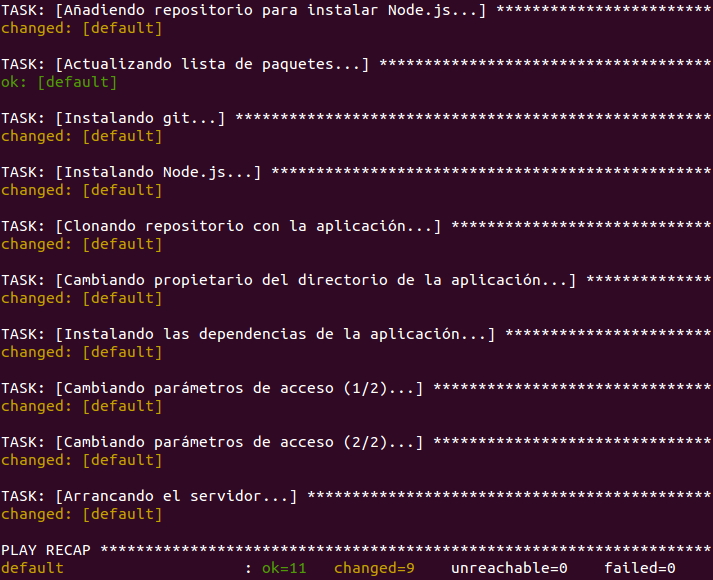
\includegraphics[width=1\textwidth]{../images/provision.png}
		\caption{Prueba de aprovisionamiento con Ansible}
		\label{fig:provision}
	\end{center}
\end{figure}

\newpage
\section{Prueba de carga}

Una vez que ya hemos realizado las pruebas de software que hemos considerado oportunas, también tenemos que pasar pruebas a la infraestructura como tal para analizar su rendimiento. En este tipo de pruebas entra en juego tanto el aspecto software como hardware con el objetivo de obtener una medición del rendimiento de nuestra aplicación.

\newpage
\subsection{Métricas y parámetros que afectan al rendimiento}

Para comparar las prestaciones de la aplicación debemos tener en cuenta los siguientes criterios:

\begin{itemize}
	\item El objetivo de esta prueba es medir las prestaciones del servidor generado por {\tt Express} para dar servicio a la aplicación del portal de transparencia bajo unas condiciones que nos aporte un análisis neutro del rendimiento del mismo.
	\item La herramienta que se usará para realizar estás mediciones es {\tt ApacheBench}.
	\item Los parámetros que se considerarán los parámetros usados en la herramienta: el número de peticiones que se realizan al servidor y el nivel de concurrencia con el que se realizan las peticiones.
	\item Los valores de estos parámetros irán modificándose para tener unos resultados más completos ante las diferentes cargas de trabajo que soportará el servidor.
\end{itemize}

El hardware y el software del sistema serán los siguientes:

\begin{itemize}
	\item \textbf{Hardware}:
	\begin{itemize}
		\item Procesador: Intel Pentium Dual CPU E2180 @ 2.00GHz
		\item Placa base: MSI MS-7255
		\item Chipset: VIA P4M900
		\item Memoria: 3GB (2+1 DIMM DDR2)
		\item Disco: Maxtor 6Y160P0 160GB 7200RPM
		\item Tarjeta gráfica: ATI Radeon X300SE 325MHz 128MB
		\item Red: Realtek RTL8100C 100Mbps
	\end{itemize}
	\item \textbf{Software}:
	\begin{itemize}
		\item Sistema operativo: Ubuntu 14.04.1 LTS i686 GNU/Linux
		\item Kernel: Linux 3.13.0-35-generic
		\item Sistema de archivos: ext4
	\end{itemize}
\end{itemize}

\newpage
\subsection{Técnicas de evaluación, carga de trabajo y diseño de experimentos}

Para evaluar el rendimiento de la aplicación vamos a realizar benchmark hacia la aplicación en ejecución para poder realizar una evaluación sobre su comportamiento bajo diferentes cargas de trabajo. El programa con el que vamos hacer las pruebas es el ya mencionado {\tt ApacheBench}, que nos permitirá realizar de forma sencilla pruebas de rendimiento a cualquier servidor, sea cual sea el lenguaje en el que esté realizado. 

\bigskip
Según la información de registros de acceso del servidor en los últimos \textbf{6 meses} el número de peticiones de páginas del portal ha sido de \textbf{2.388 peticiones}, lo que sería aproximadamente \textbf{13 peticiones/día}. Para realizar los diferentes tests se realizará un \textbf{número de conexiones} variables al servidor (\textbf{30, 50 y 100}) con diferentes \textbf{niveles de concurrencia} en función del total de conexiones (\textbf{25\%, 50\% y 75\%}). Los números de conexiones para las prueba han sido elegidos para evaluar como se comportaría el servidor ante un gran aumento de actividad en el mismo en línea con el nivel de conexiones que se producen en la actualidad.

\bigskip
De entre las peticiones al portal, la página que ha recibido un mayor número de peticiones es la página de \textbf{Personal}, por lo que el experimento a realizar consistirá en realizar peticiones de la página de \textbf{Personal} a la aplicación. Este experimente nos permitirá comprobar como se comportará la aplicación en diferentes situaciones cono diferentes niveles de carga y la repercusión en su rendimiento ante estás diferentes pruebas, viendo por ejemplo si fuera necesario buscar una forma de balancear la carga del servidor. 

\bigskip
En total el experimento constará de 9 pruebas, y a su vez cada una de estas pruebas se repetirá 10 veces consecutivas para así asegurarnos que los resultados son legítimos y no producto de sucesos fortuitos. Los resultados mostrados serán la media de esas 10 ejecuciones y su desviación estándar, que nos permitirá saber como de válidos podemos considerar los valores medios obtenidos. Estos valores promedios se introducirán en un gráfico para comparar los cambios que se producen con diferentes números de conexiones y mismos porcentaje de concurrencia. Las variables respuestas a tener en cuenta para el estudio serán:

\begin{itemize}
	\item Tiempo de ejecución.
	\item Solicitudes por segundo.
	\item Tiempo por solicitud concurrente.
	\item Velocidad de transferencia.
\end{itemize}

\bigskip
El único factor a considerar para el experimento será, como hemos
dicho, las respuestas del servidor de la aplicación desarrollada del
portal de transparencia {\tt UGR Transparente}. Cuando se disponga de
los resultados de todas las pruebas, se procederá a analizar e
interpretar los resultados. % ¿Y cuando se va a disponer? - JJ

\subsection{Presentación de los resultados}

Enumeración de las pruebas a realizar en el experimento:

\begin{itemize}
	\item \textbf{Prueba 1}: 30 solicitudes, concurrencia del 25\% (8).
	\item \textbf{Prueba 2}: 30 solicitudes, concurrencia del 50\% (15).
	\item \textbf{Prueba 3}: 30 solicitudes, concurrencia del 75\% (23).
	\item \textbf{Prueba 4}: 50 solicitudes, concurrencia del 25\% (13).
	\item \textbf{Prueba 5}: 50 solicitudes, concurrencia del 50\% (25).
	\item \textbf{Prueba 6}: 50 solicitudes, concurrencia del 75\% (38).
	\item \textbf{Prueba 7}: 100 solicitudes, concurrencia del 25\% (25).
	\item \textbf{Prueba 8}: 100 solicitudes, concurrencia del 50\% (50).
	\item \textbf{Prueba 9}: 100 solicitudes, concurrencia del 75\% (75).
\end{itemize}

\subsubsection{Tiempo de ejecución}
\begin{table}[!ht]
	\begin{center}
		\begin{tabular}{|c|c|c|c|}
			\hline
			\multicolumn{4}{|c|}{{\bf Tiempo de ejecución}}                                                           \\ \hline
			{\bf N.º conexiones} & {\bf Concurrencia (\%)} & {\bf Segundos} & {\bf Desviación} \\ \hline
			{\it 30}                   & {\it 25}                  & 8,823              & 0,199                     \\ \hline
			{\it 30}                   & {\it 50}                  & 7,552              & 0,214                     \\ \hline
			{\it 30}                   & {\it 75}                  & 6,827              & 0,970                     \\ \hline
			{\it 50}                   & {\it 25}                  & 10,215             & 0,248                     \\ \hline
			{\it 50}                   & {\it 50}                  & 12,506             & 0,299                     \\ \hline
			{\it 50}                   & {\it 75}                  & 13,959             & 0,217                     \\ \hline
			{\it 100}                  & {\it 25}                  & 26,966             & 1,781                     \\ \hline
			{\it 100}                  & {\it 50}                  & 22,850             & 3,845                     \\ \hline
			{\it 100}                  & {\it 75}                  & 24,473             & 3,845                     \\ \hline
		\end{tabular}
		\caption{Resultados de tiempo de ejecución}
		\label{table:rte}
	\end{center}
\end{table}

\begin{figure}[!ht]
	\begin{center}
		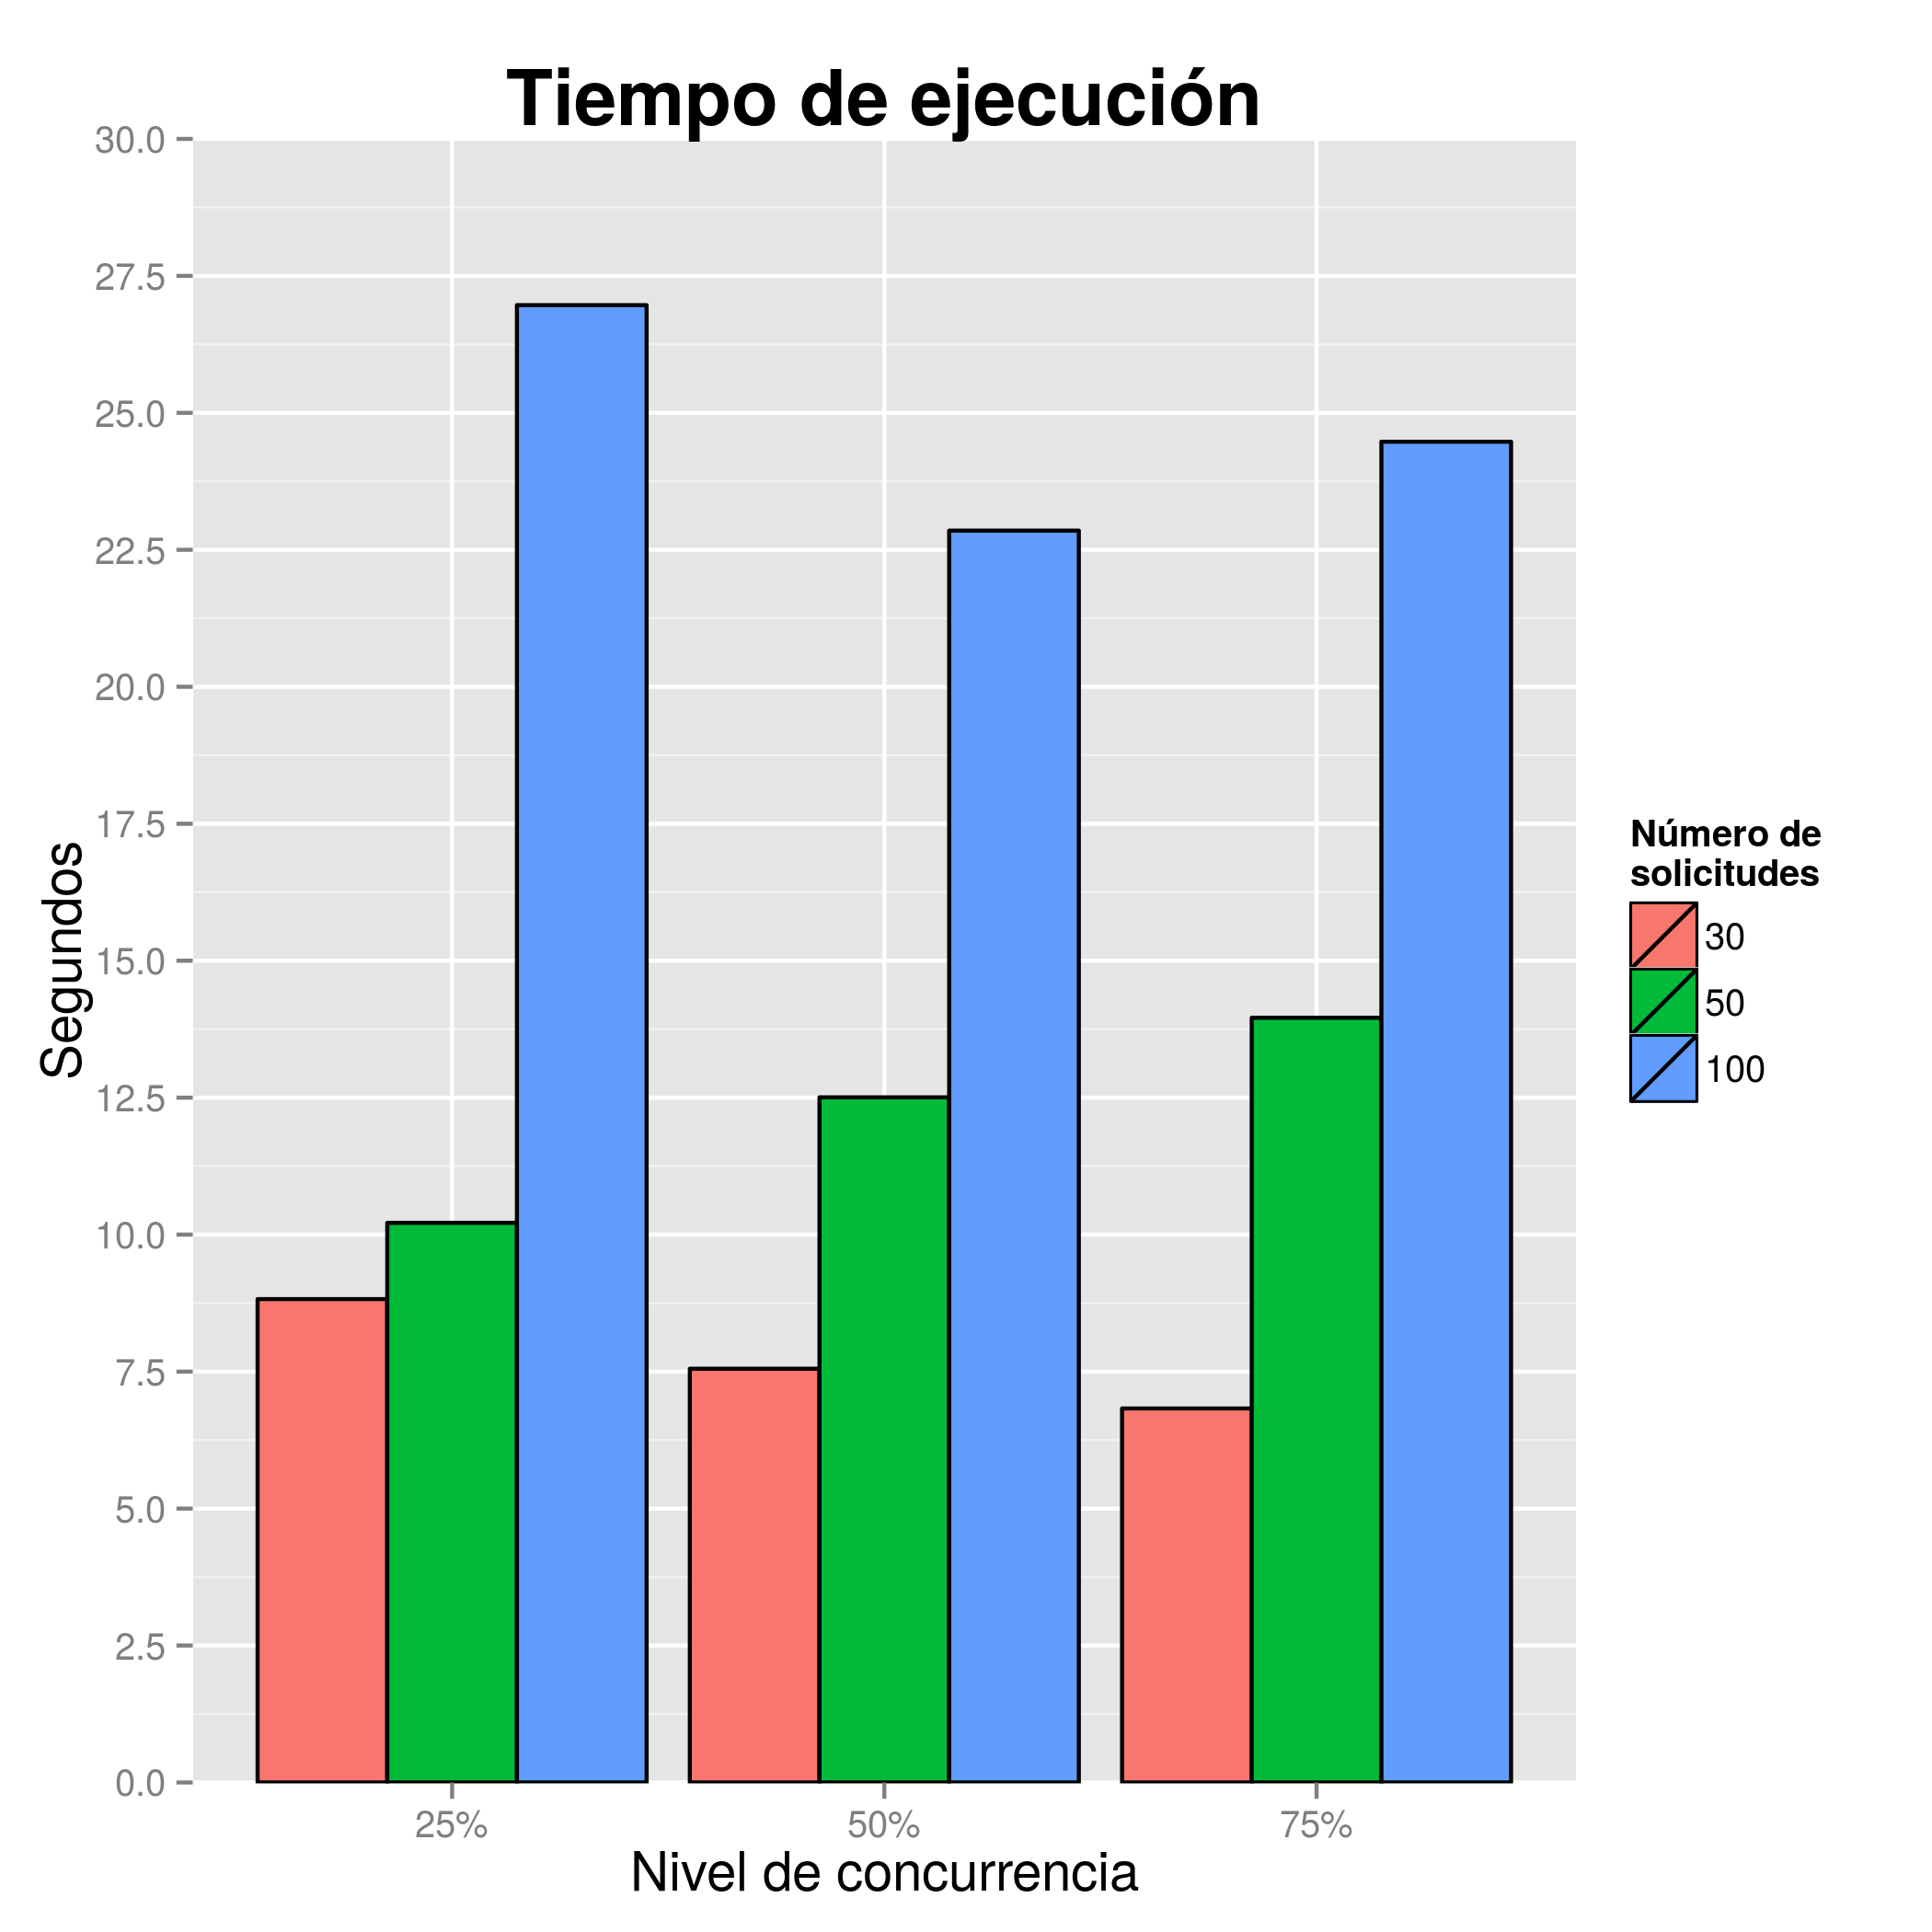
\includegraphics[width=0.8\textwidth]{../graphics/gra_te.png}
		\caption{Gráfico de tiempo de ejecución}
		\label{fig:gra_te}
	\end{center}
\end{figure}

\newpage
\subsubsection{Solicitudes por segundo}
\begin{table}[!ht]
	\begin{center}
		\begin{tabular}{|c|c|c|c|}
			\hline
			\multicolumn{4}{|c|}{{\bf Solicitudes por segundo}}                                                   \\ \hline
			{\bf N.º de conexiones} & {\bf Concurrencia (\%)} & {\bf Solicitudes/s} & {\bf Desviación} \\ \hline
			{\it 30}                & {\it 25}                & 3,402                          & 0,078            \\ \hline
			{\it 30}                & {\it 50}                & 3,976                          & 0,113            \\ \hline
			{\it 30}                & {\it 75}                & 4,470                          & 0,531            \\ \hline
			{\it 50}                & {\it 25}                & 4,898                          & 0,118            \\ \hline
			{\it 50}                & {\it 50}                & 4,000                          & 0,095            \\ \hline
			{\it 50}                & {\it 75}                & 3,583                          & 0,056            \\ \hline
			{\it 100}               & {\it 25}                & 3,728                          & 0,292            \\ \hline
			{\it 100}               & {\it 50}                & 4,496                          & 0,708            \\ \hline
			{\it 100}               & {\it 75}                & 4,197                          & 0,703            \\ \hline
		\end{tabular}
		\caption{Resultados de solicitudes por segundo}
		\label{table:rss}
	\end{center}
\end{table}

\begin{figure}[!ht]
	\begin{center}
		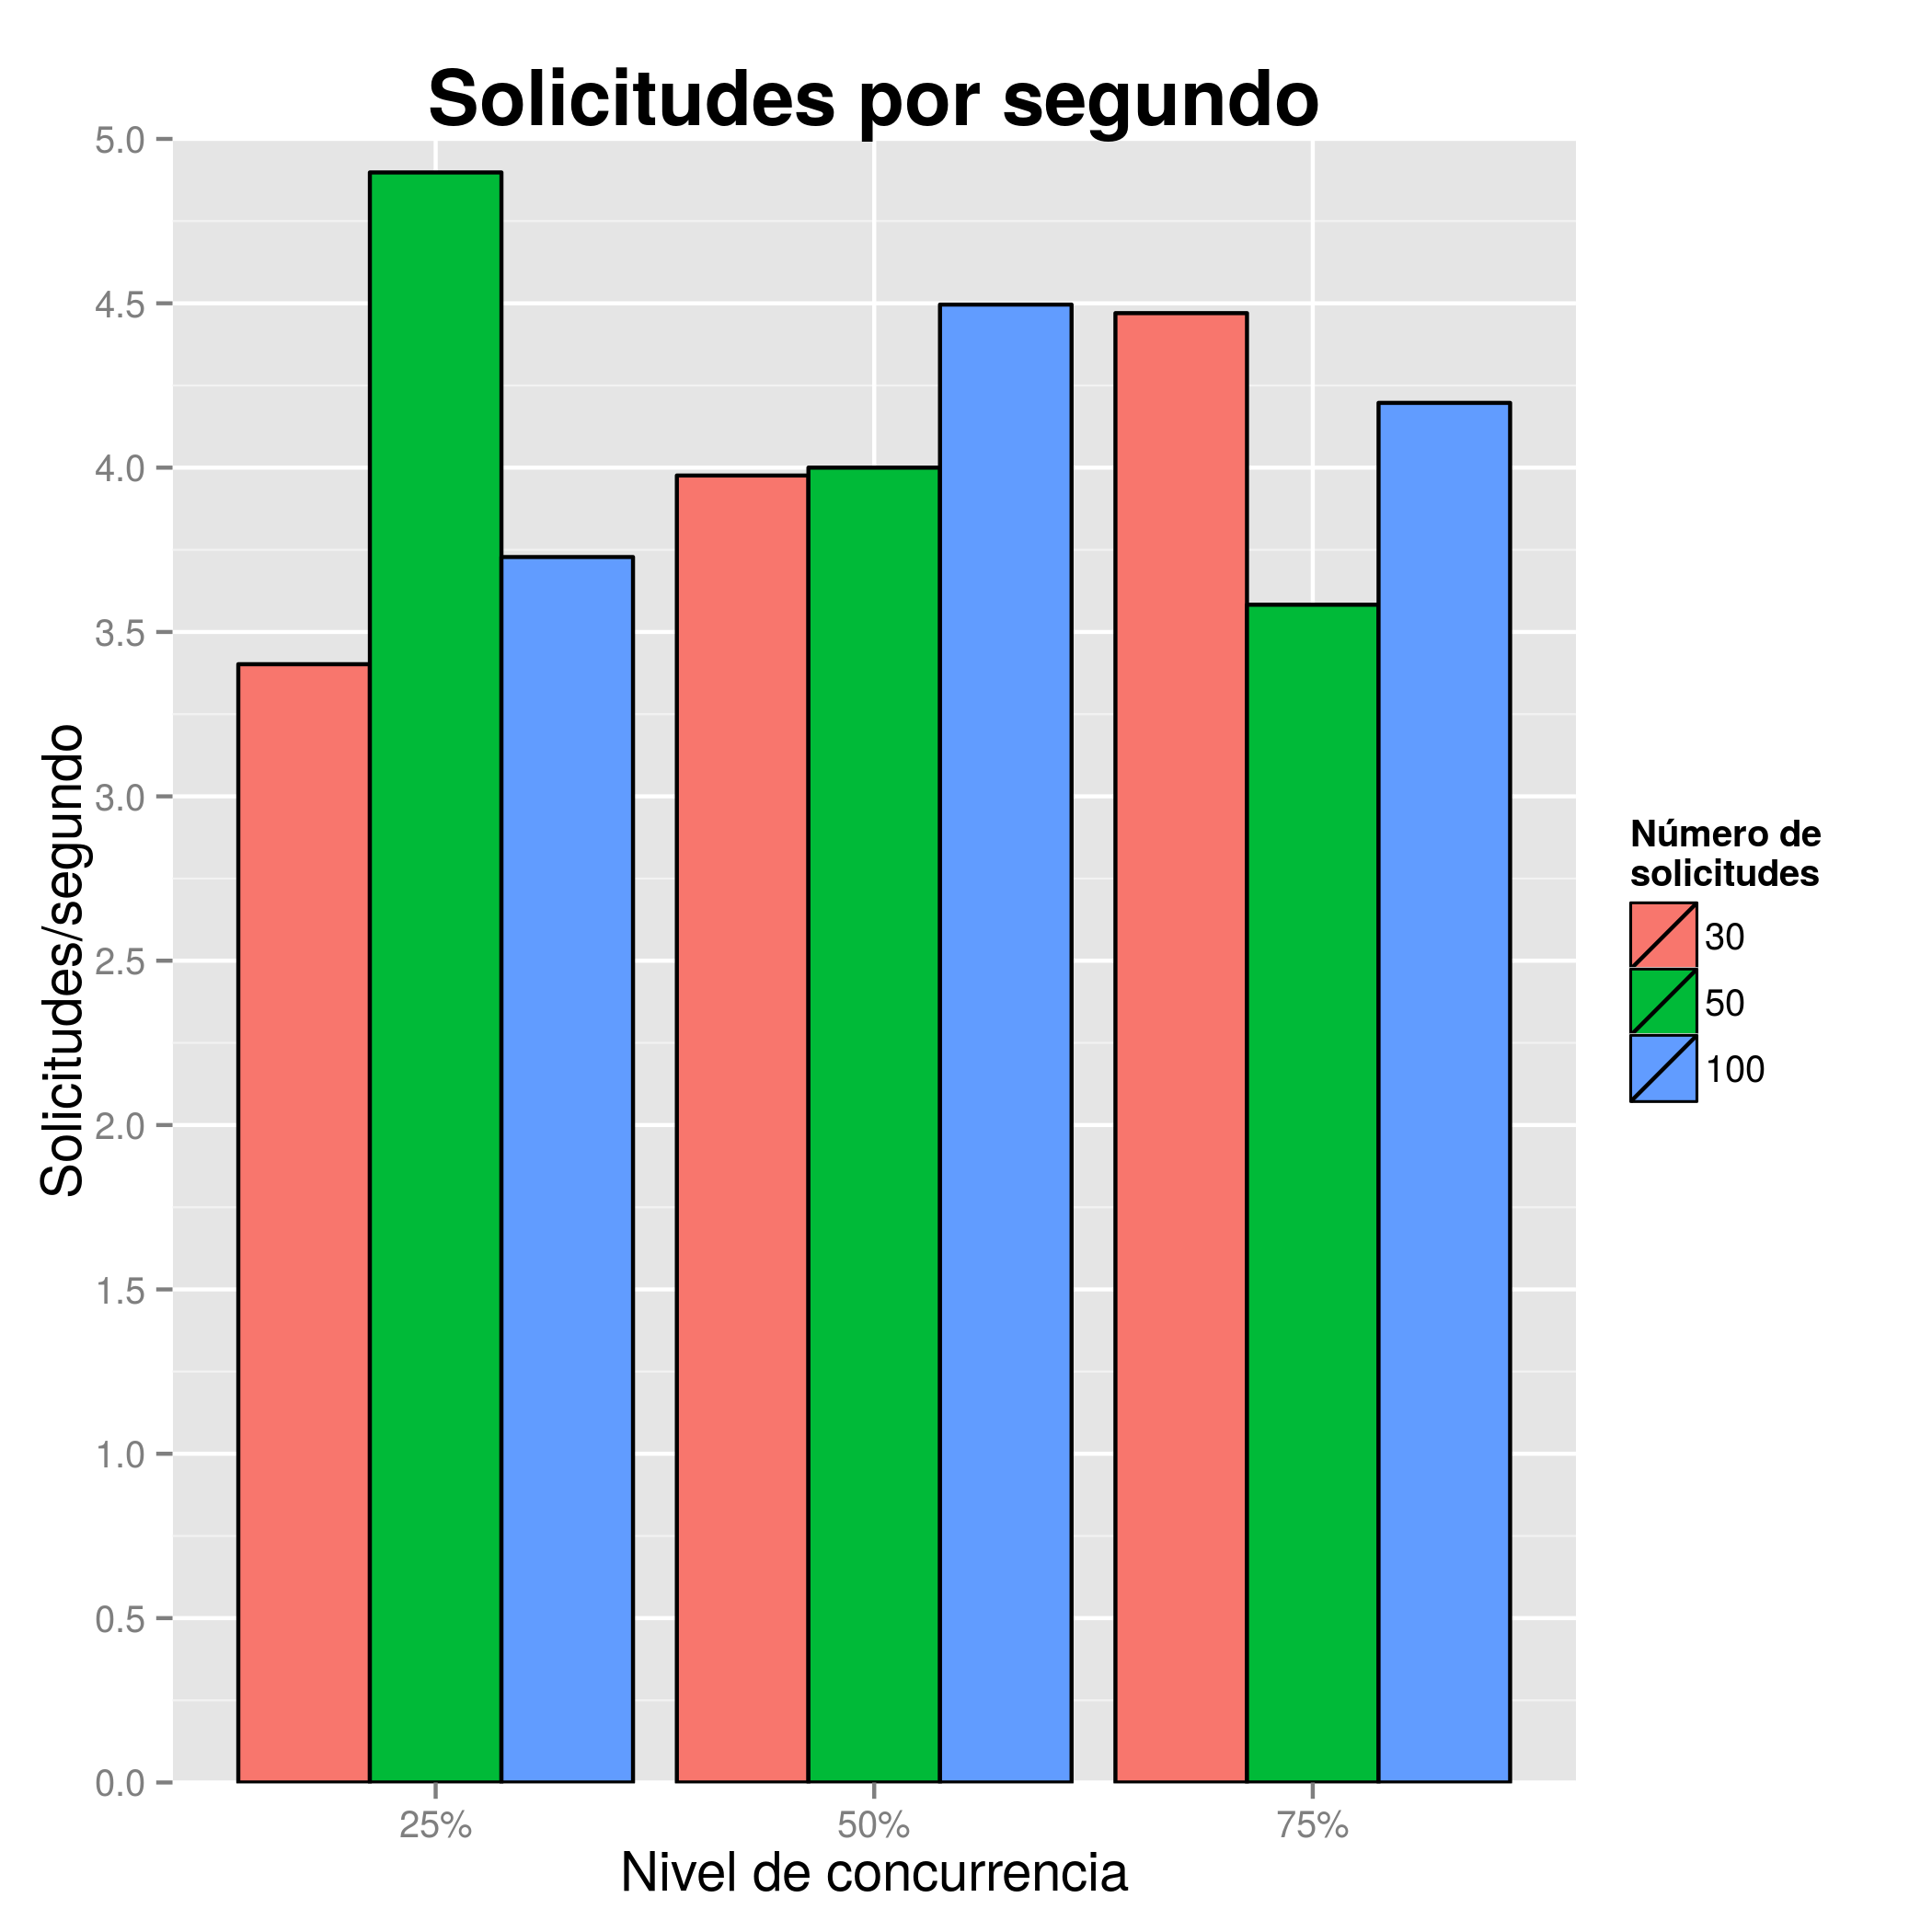
\includegraphics[width=0.8\textwidth]{../graphics/gra_sps.png}
		\caption{Gráfico de solicitudes por segundo}
		\label{fig:gra_sps}
	\end{center}
\end{figure}

\newpage
\subsubsection{Tiempo por solicitud concurrente}
\begin{table}[!ht]
	\begin{center}
		\begin{tabular}{|c|c|c|c|}
			\hline
			\multicolumn{4}{|c|}{{\bf Tiempo por solicitud concurrente}}                               \\ \hline
			{\bf N.º de conexiones} & {\bf Concurrencia (\%)} & {\bf Promedio (ms)} & {\bf Desviación} \\ \hline
			{\it 30}                & {\it 25}                & 294,087             & 6,645            \\ \hline
			{\it 30}                & {\it 50}                & 251,733             & 7,129            \\ \hline
			{\it 30}                & {\it 75}                & 227,563             & 32,347           \\ \hline
			{\it 50}                & {\it 25}                & 204,296             & 4,959            \\ \hline
			{\it 50}                & {\it 50}                & 250,128             & 5,990            \\ \hline
			{\it 50}                & {\it 75}                & 279,178             & 4,346            \\ \hline
			{\it 100}               & {\it 25}                & 269,658             & 17,811           \\ \hline
			{\it 100}               & {\it 50}                & 228,497             & 38,451           \\ \hline
			{\it 100}               & {\it 75}                & 244,729             & 38,449           \\ \hline
		\end{tabular}
		\caption{Resultados de tiempo por solicitud concurrente}
		\label{table:rtsc}
	\end{center}
\end{table}

\begin{figure}[!ht]
	\begin{center}
		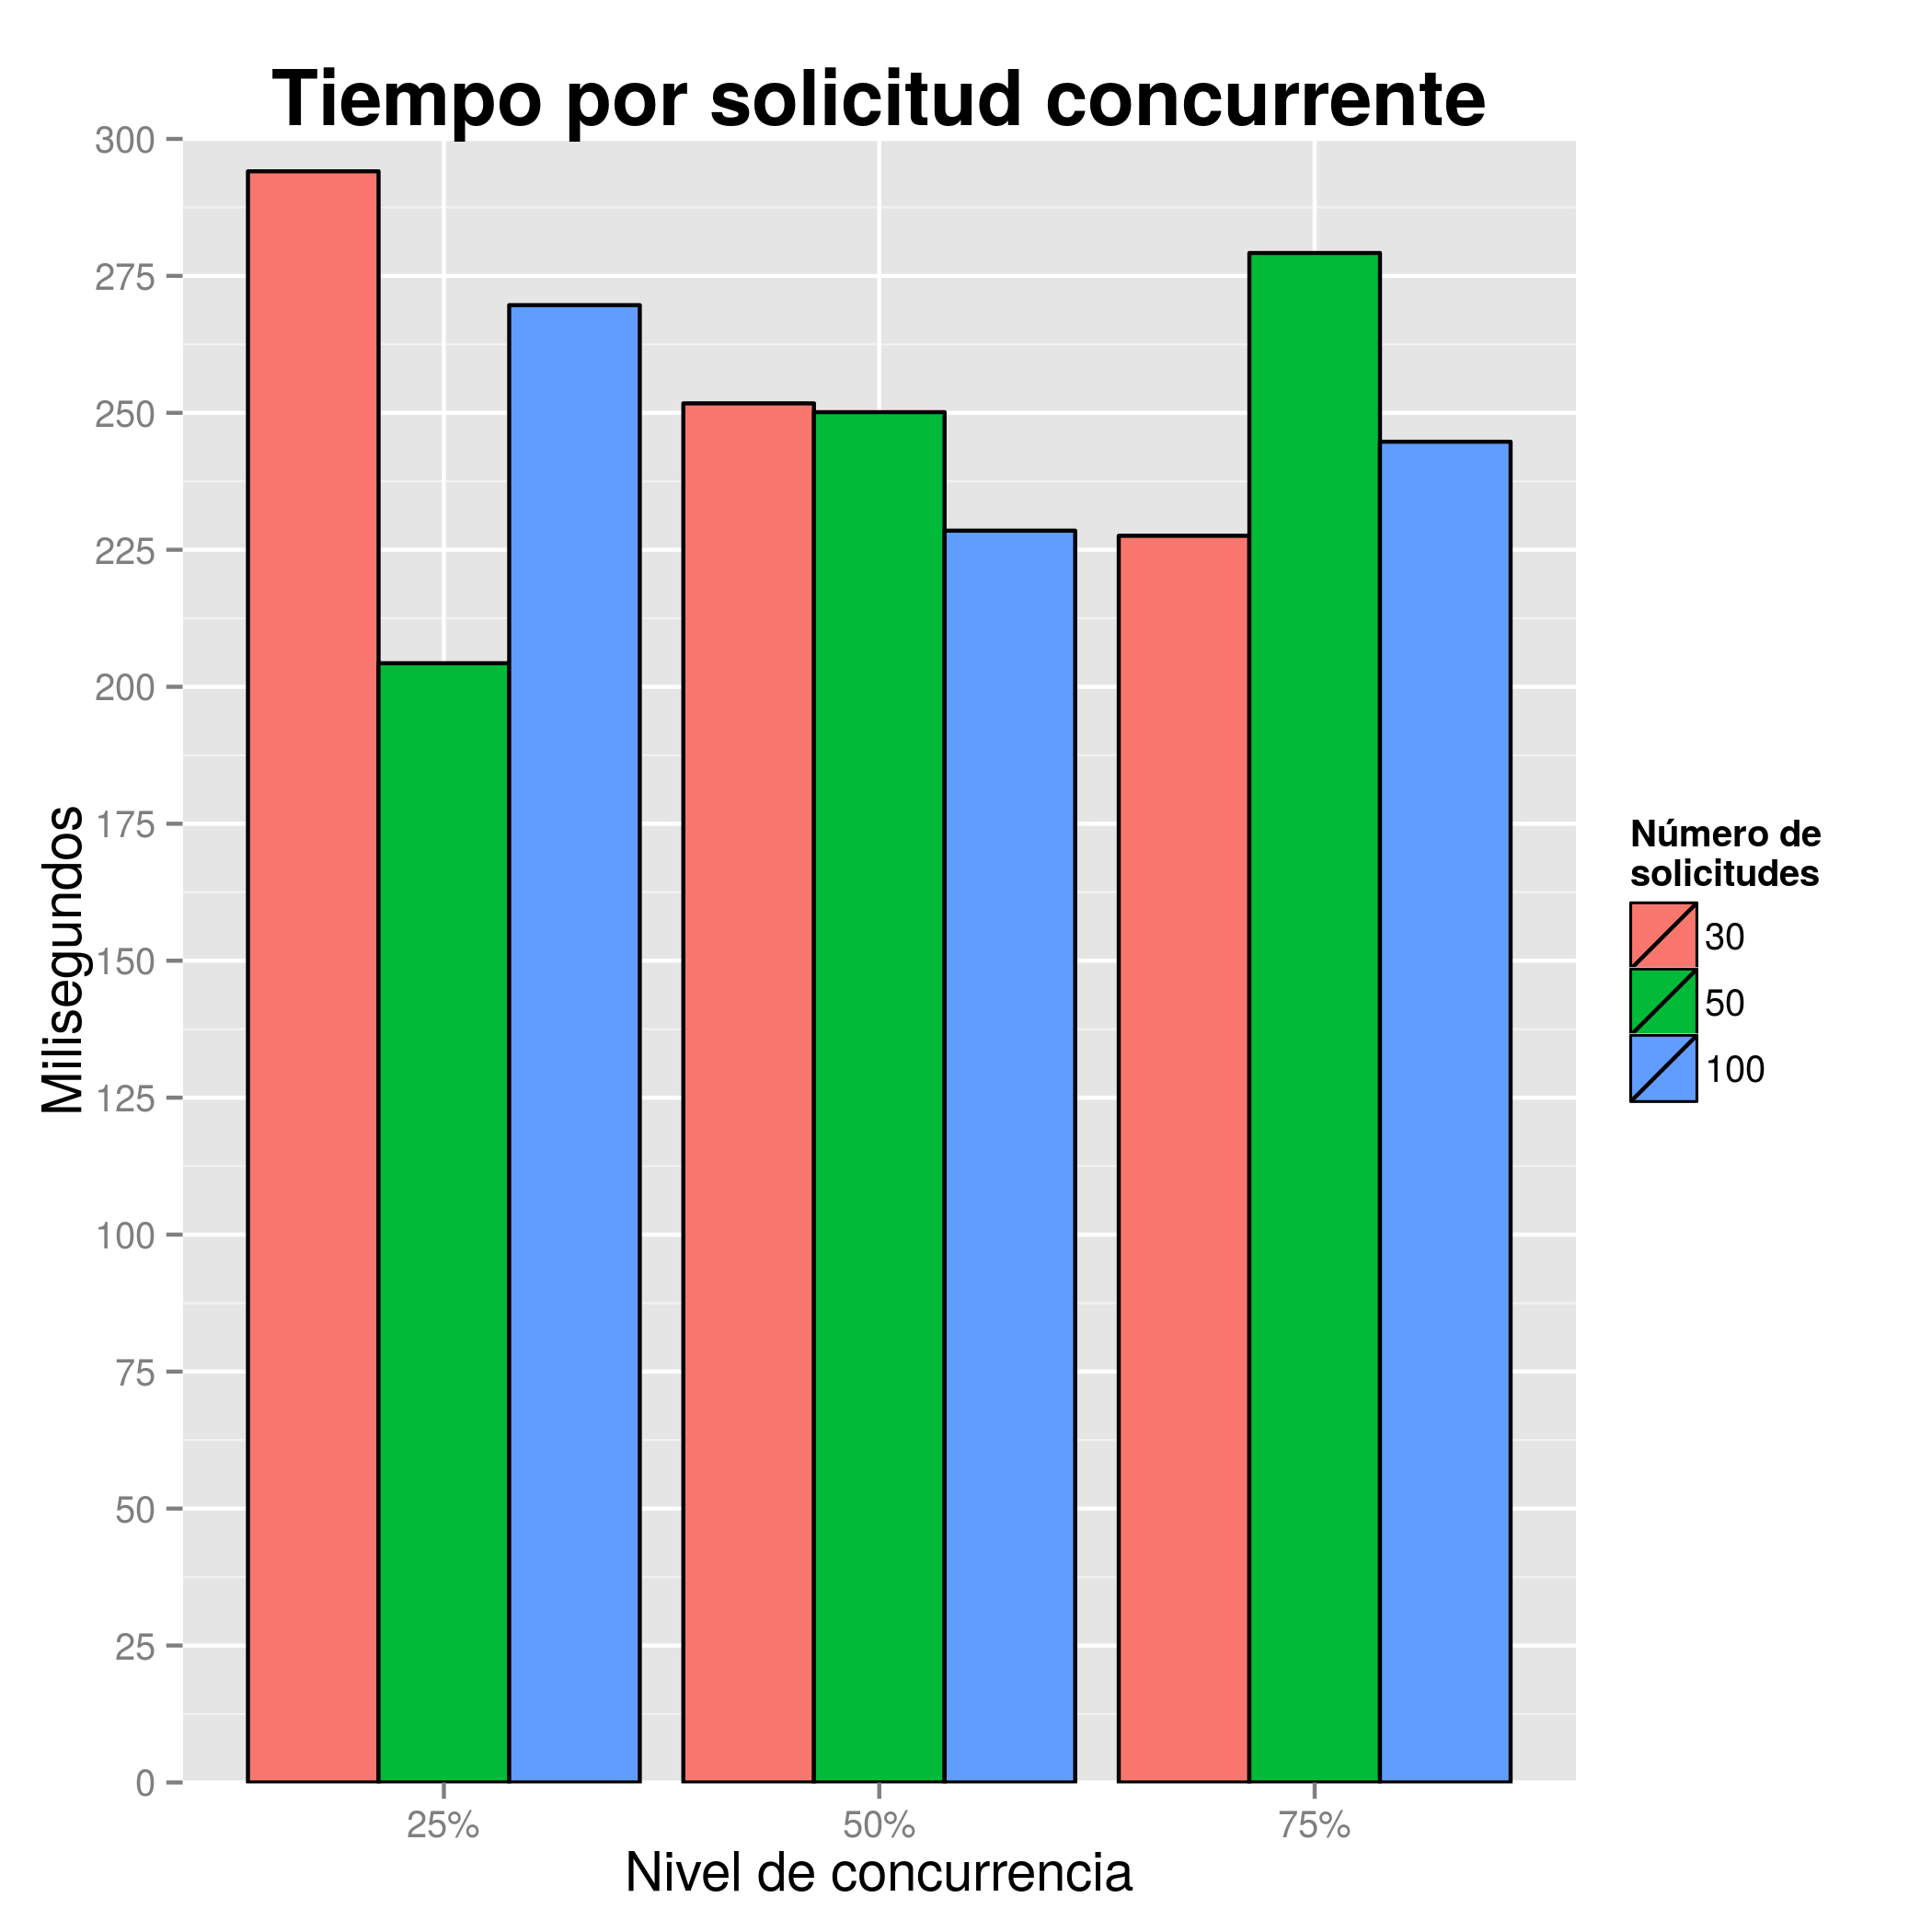
\includegraphics[width=0.8\textwidth]{../graphics/gra_tsc.png}
		\caption{Gráfico de tiempo por solicitud concurrente}
		\label{fig:gra_tsc}
	\end{center}
\end{figure}

\newpage
\subsubsection{Velocidad de transparencia}
\begin{table}[!ht]
	\begin{center}
		\begin{tabular}{|c|c|c|c|}
			\hline
			\multicolumn{4}{|c|}{{\bf Velocidad de transferencia}}                            \\ \hline
			{\bf N.º de conexiones} & {\bf Concurrencia (\%)} & {\bf KB/s} & {\bf Desviación} \\ \hline
			{\it 30}                & {\it 25}                & 747,735    & 17,116           \\ \hline
			{\it 30}                & {\it 50}                & 873,789    & 24,798           \\ \hline
			{\it 30}                & {\it 75}                & 982,389    & 116,778          \\ \hline
			{\it 50}                & {\it 25}                & 645,866    & 15,498           \\ \hline
			{\it 50}                & {\it 50}                & 527,515    & 12,561           \\ \hline
			{\it 50}                & {\it 75}                & 472,469    & 7,339            \\ \hline
			{\it 100}               & {\it 25}                & 245,783    & 19,227           \\ \hline
			{\it 100}               & {\it 50}                & 296,416    & 46,684           \\ \hline
			{\it 100}               & {\it 75}                & 276,707    & 46,384           \\ \hline
		\end{tabular}
		\caption{Resultados de velocidad de transferencia}
		\label{table:rvt}
	\end{center}
\end{table}

\begin{figure}[!ht]
	\begin{center}
		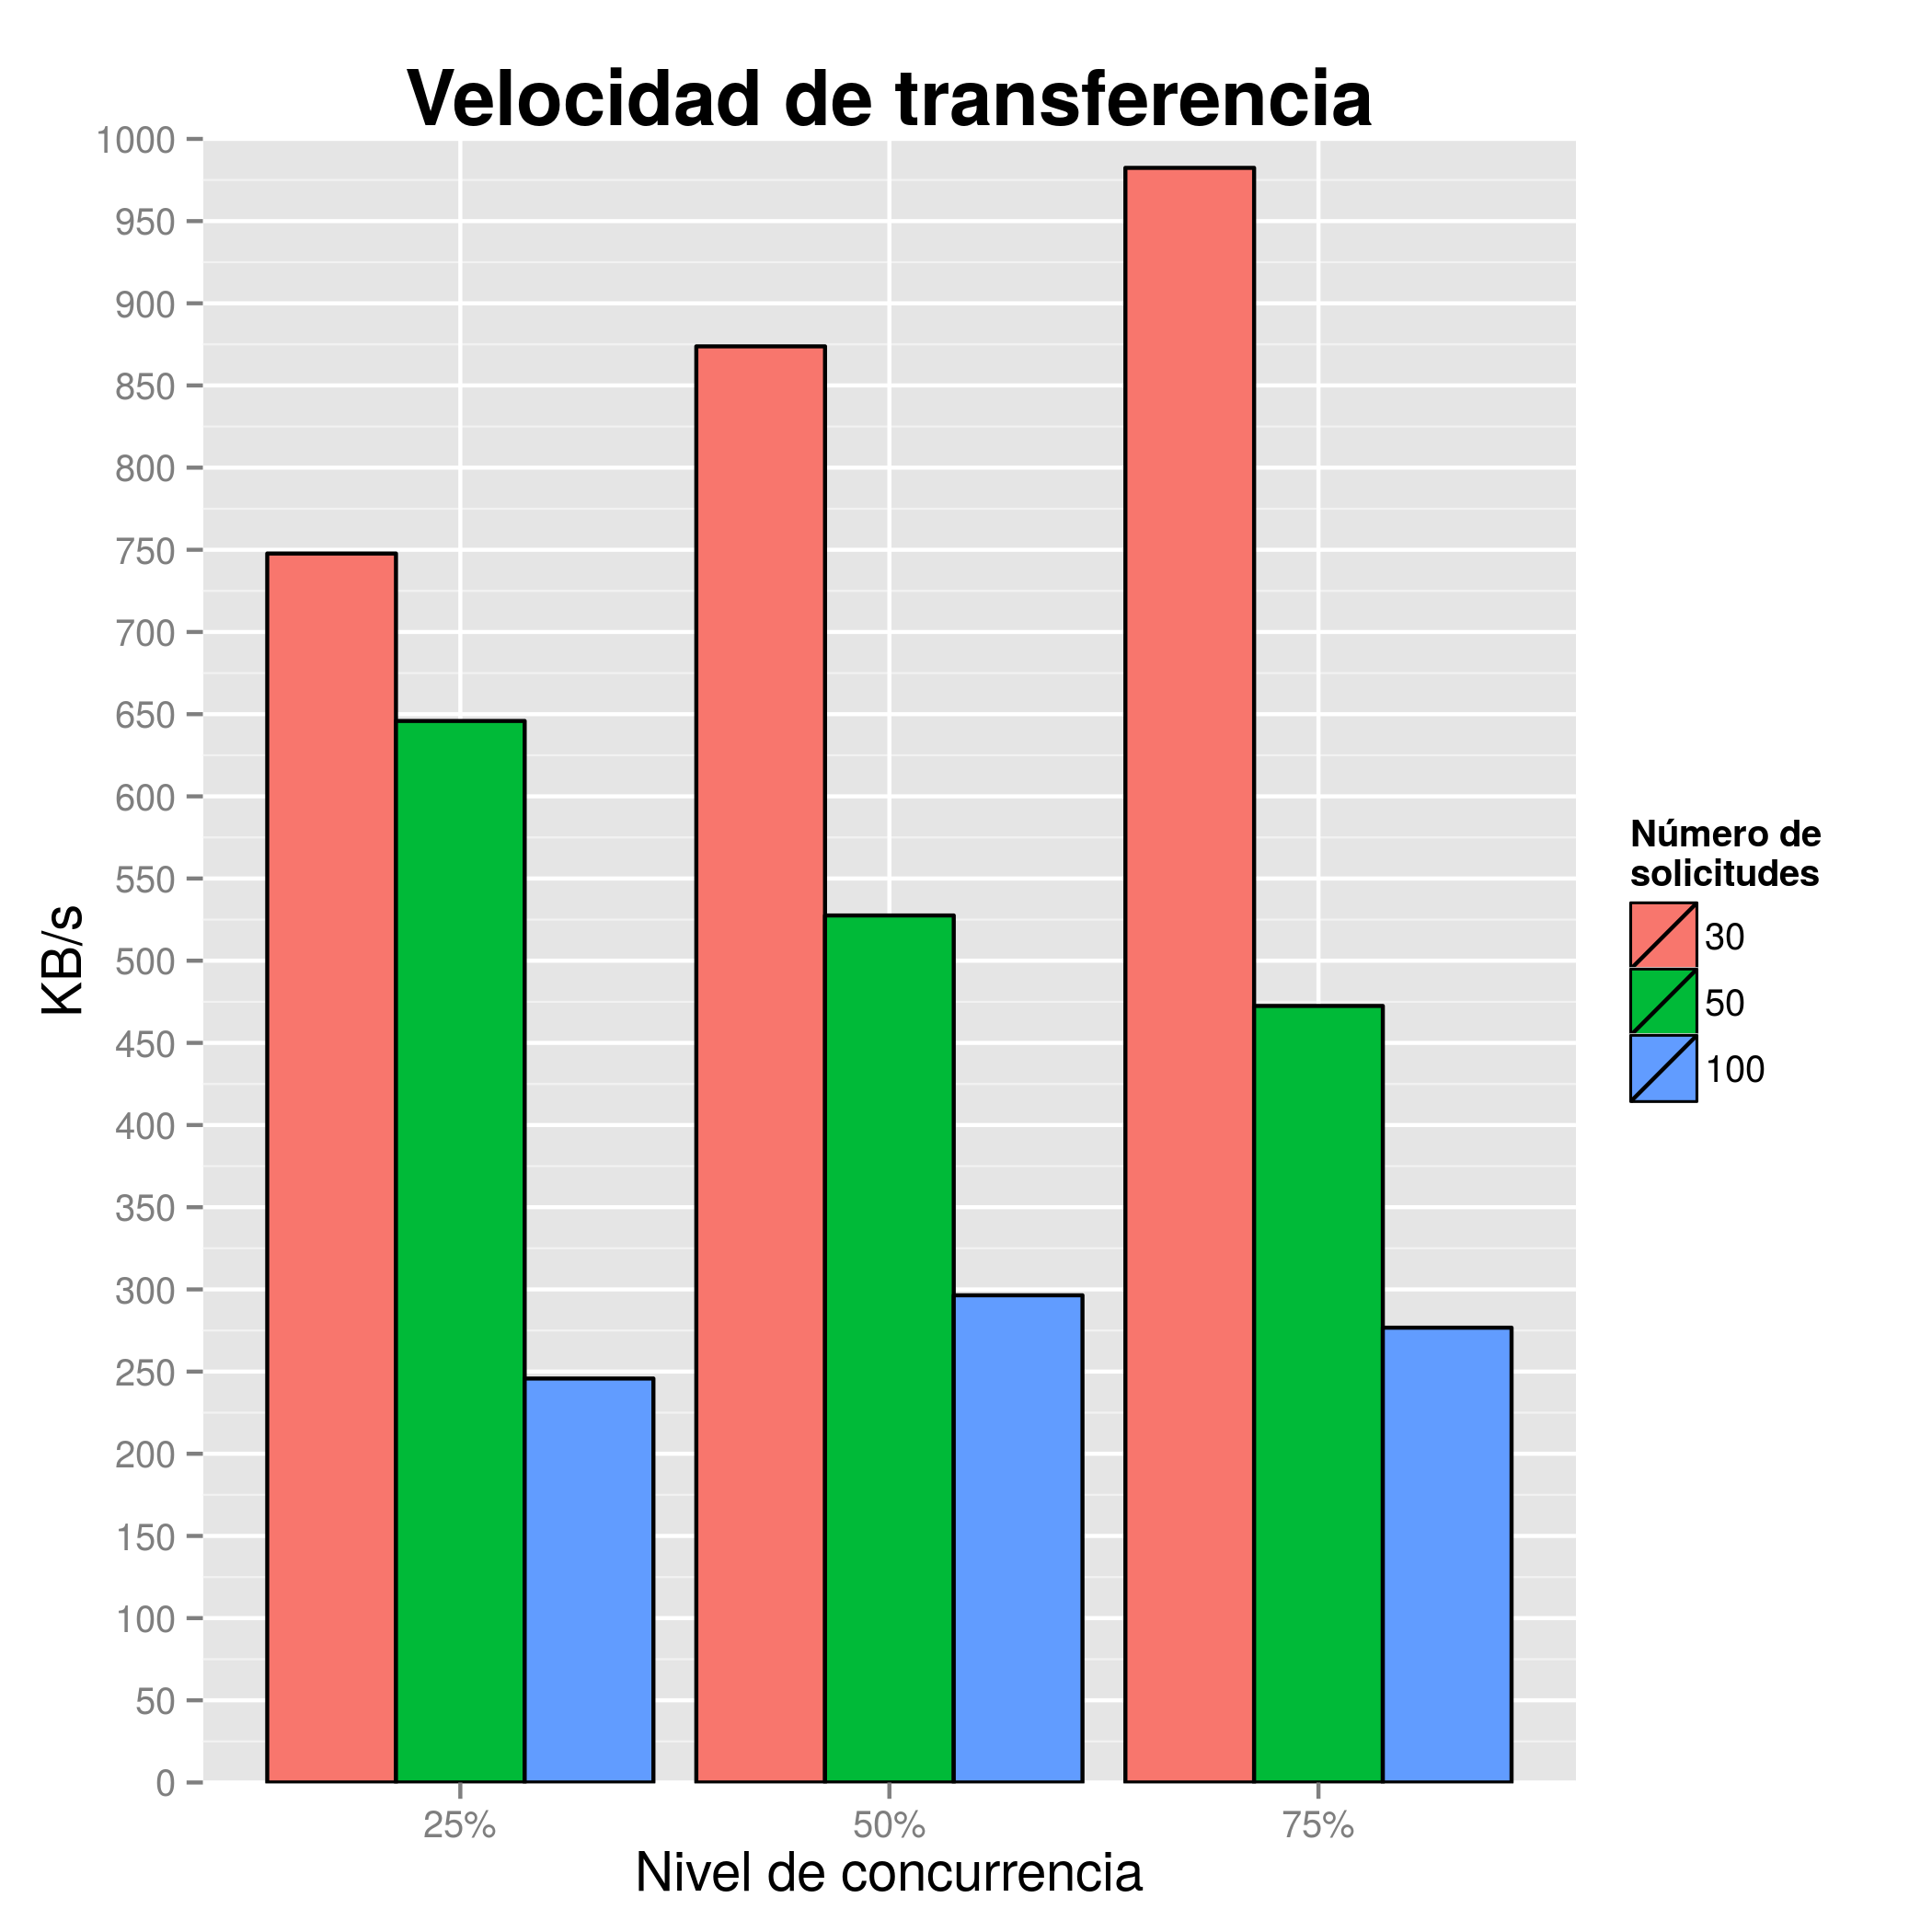
\includegraphics[width=0.8\textwidth]{../graphics/gra_vt.png}
		\caption{Gráfico de velocidad de transferencia}
		\label{fig:gra_vt}
	\end{center}
\end{figure}

\newpage
\subsection{Análisis e interpretación de los resultados}

\subsubsection{Tiempo de ejecución}
\begin{itemize}
	\item Para un número de 30 conexiones (poco más de la media de conexiones diarias al portal) la concurrencia no afecta al tiempo de respuesta de la aplicación.
	\item Cuando el número de conexiones aumenta hasta 50, vemos como en este el nivel de concurrencia sí empieza a afectar al tiempo de respuesta de la aplicación de forma negativa.
	\item En la última prueba con un número de conexiones bastante más elevado, vemos en los tiempos de ejecución que el comportamiento es más aleatorio. Si nos fijamos en las desviaciones estás han crecido bastante en comparación con las pruebas anteriores, por lo que aparentemente la aplicación empieza a soportar cierta sobrecarga.
\end{itemize}

\subsubsection{Solicitudes por segundo}
\begin{itemize}
	\item En relación directa con los resultados descritos en el apartado anterior vemos que para 30 conexiones, al igual que el tiempo de respuesta bajaba según el nivel de concurrencia, ahora el número de solicitudes respondidas por segundo aumentan; el comportamiento que cabría esperar.
	\item En el caso de 50 conexiones, de igual forma, cuando el nivel de concurrencia sube, el número de solicitudes respondidas baja.
	\item Para la prueba de 100 conexiones volvemos a tener una situación similar a la anterior, donde aunque en esta caso las desviaciones no son tan altas, no se puede concretar una tendencia en el rendimiento de la aplicación.
\end{itemize}

\subsubsection{Tiempo por solicitud concurrente}
\begin{itemize}
	\item Se produce la misma situación, para 30 conexiones el tiempo necesario para resolver una solicitud recurrente va disminuyendo según aumenta la concurrencia en las conexiones. A destacar que en esta prueba el valor de la desviación crece en gran cantidad, por lo que aunque se puede encontrar una tendencia general de mejor en el rendimiento los tiempos para resolver las solicitudes no son tan homogéneos.
	\item En el caso de las 50 conexiones también se produce la misma situación a las pruebas anteriores: según aumenta la concurrencia aumenta el tiempo necesario para responder una solicitud concurrente, lo que indica que el rendimiento ha bajado.
	\item De igual forma, para 100 conexiones volvemos a encontrar sin un patrón claro de comportamiento, pero si podemos destacar que las desviaciones son enormes.
\end{itemize}

\subsubsection{Velocidad de transferencia}
\begin{itemize}
	\item Mismo patrón para la prueba con 30 conexiones. Habíamos visto que según aumenta la concurrencia, disminuye el tiempo de ejecución y aumentan el número de solicitudes por segundo respondidas o lo que es lo mismo, aumenta el rendimiento; así que como podríamos intuir y con estos datos comprobar, también aumenta la cantidad de información transferida. Nos encontramos en algunos casos con desviaciones enormes, pero eso podemos atribuirlo a la propia naturaleza inestable de las conexiones de red.
	\item Como se ha venido produciendo, en el caso de la prueba con 50 conexiones el rendimiento ha ido bajando según ha ido aumentando el porcentaje de concurrencia; esto también se produce en este caso: según aumentaba la concurrencia, disminuía la velocidad de transferencia.
	\item Por último, en la prueba con 100 conexiones esta es la prueba que ha tenido resultados más igualados (y además muy bajos en comparación) entre los diferentes niveles de concurrencia, lo que nos vuelve a hacer suponer que el servidor está sobrecargado.
\end{itemize}

\subsection{Conclusiones sobre los resultados}

Una vez analizados los resultados de las pruebas realizadas la conclusión a la que podríamos llegar
es que la aplicación puede aguantar perfectamente la carga de trabajo que tiene en la actualidad (alrededor de 13 peticiones al día), y que tampoco no habría ningún problema en que esta se duplicara como hemos visto en los resultados de las pruebas de 30 conexiones. El problema aparecería si este volumen de visitas siguiera creciendo, ya que como hemos visto en las pruebas de 50 conexiones, en cuanto empieza a aumentar la concurrencia de las solicitudes el rendimiento de la aplicación cae, llegando a un punto de las pruebas de 100 conexiones en el la aplicación comienza a estar sobrecargada.

\bigskip
Viendo el volumen de visitas actual, es dificil que a corto plazo se llegarán a producir este tipo de problemas de saturación, sin embargo, en futuro se deberían aplicar técnicas de balanceo de carga sobre la aplicación usando algún otro módulo de {\tt Node.js} como puede ser {\tt node-http-proxy}, cambiar la estructura de la aplicación para que esta no tenga problemas a unos niveles altos de carga de trabajo, o incluso cambiar el sistema operativo por otro que pudiera dar un mayor rendimiento en entornos de servidores.

\section{Acceso web}

El resultado final es que el portal de transparencia sigue siendo accesible, y aunque visualmente no se aprecia ningún cambio, por debajo su funcionamiento y su desarrollo han cambiado completamente a como se ha descrito a lo largo de todo el documento.

\begin{figure}[!ht]
	\begin{center}
		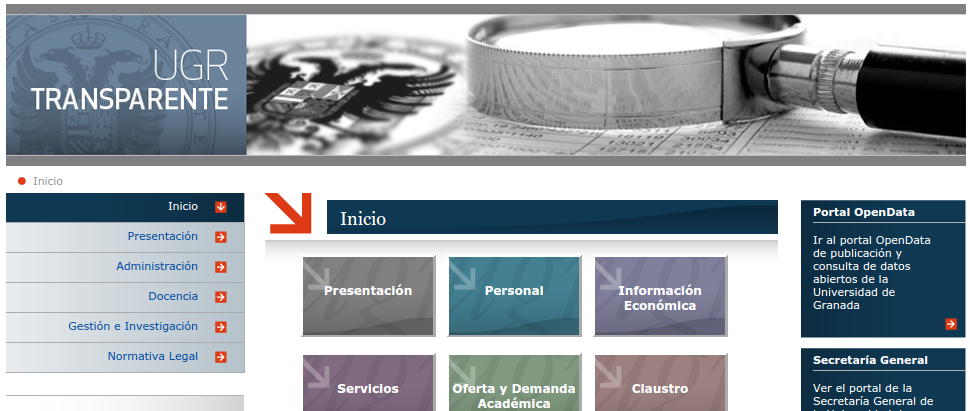
\includegraphics[width=1\textwidth]{../images/transparente.png}
		\caption{Visualización del portal de transparencia}
		\label{fig:transparente}
	\end{center}
\end{figure}
%
%\chapter{Conclusiones y trabajos futuros}

Después de realizar este proyecto la principal conclusión a la que se puede llegar es que si bien un desarrollado menos \textit{instrumentado} puede ser muy rápido, el dividir el desarrollo en diferentes etapas (con herramientas que a su vez tienen sus propios sistemas de control) harán del desarrollo una tarea más fácil y robusta.

\bigskip
Este era uno de los principales problemas del estado inicial del portal, al no encontrarse por ejemplo implementados ningún tipo de tests unitarios se producían varios errores por causas desconocidas que eran difíciles de situar en el código de la aplicación.

\bigskip
Uno de los principales problemas, es que para esta metodología de desarrollo las fases de planificación y análisis pueden ser más difíciles de plantear, ya que se basa en un desarrollo continuo en el que todo elemento a desarrollar se decide según la necesidad y generalmente con un tiempo de antelación bastante corto.

\bigskip
Como ventaja tenemos que hay un gran cantidad de herramientas para gestionar las diferentes etapas, pudiendo elegir las que consideremos precisas en un determinado momento ya sea por restricciones del desarrollo o por simple comodidad. Por ejemplo: los test unitarios se podrían haber pasado con {\tt Unit JS}, la integración continua con {\tt Jenkins} y el provisionamiento con {\tt Chef}; así aunque los procedimientos fueran distintos, el resultado hubiera sido el mismo.

\newpage
En cuanto a trabajos futuros relacionados con el proyecto algunas posibilidades serían:

\begin{itemize}
	\item Realizar un instalación personalizada de {\tt CKAN} en un versión actual de {\tt Ubuntu} (actualmente solo existe una instalación oficial para la versión 12.04) para poder desarrollar
	plugins propios con el fin de realizar tareas que se puedan considerar interesantes; principalmente interesa que los datos se pudieran obtener directamente desde el propio {\tt CKAN} y no se tuvieran que introducir manualmente mediante archivos \textit{JSON}.
	\item Sería conveniente hacer que en general el portal sea más dinámico porque actualmente todas las páginas son estáticas, si eso se mantiene así en unos cuantos años cuando la cantidad de datos disponibles aumente considerablemente, la navegabilidad por el portal empeorará considerablemente. Sería necesario implementar un forma de que se puedan seleccionar para visualizar solo los datos que se deseen.
	\item Analizando los resultados de las pruebas de carga observamos que cuando el número de peticiones aumentaba en gran cantidad con respecto a la carga de trabajo actual, o aunque las peticiones no aumentaran tanto, pero si aumentase el nivel de concurrencia la aplicación se saturaba. Estoy debería ser solucionado mediante cambios en las estructura de la aplicación o uso de balanceo de carga.
\end{itemize}
%
%%\chapter{Conclusiones y Trabajos Futuros}
%
%
%%\nocite{*}
%\bibliography{bibliografia/bibliografia}\addcontentsline{toc}{chapter}{Bibliografía}
%\bibliographystyle{miunsrturl}
%
%\appendix
%\input{apendices/manual_usuario/manual_usuario}
%%\input{apendices/paper/paper}
%\input{glosario/entradas_glosario}
% \addcontentsline{toc}{chapter}{Glosario}
% \printglossary
\chapter*{}
\thispagestyle{empty}

\end{document}
